\documentclass[9pt,a4paper]{article}
% ============================================================
% Atlas / HOLOGY 9.0 HoloDev proposal - shared preamble
% MGM Laboratory design system, ported to LaTeX (tectonic -X)
% ============================================================

\usepackage[a4paper,top=2.1cm,bottom=2.3cm,left=2.15cm,right=2.15cm,headheight=26pt,headsep=16pt,footskip=32pt]{geometry}

% ---------- Fonts ----------
\usepackage{fontspec}
\defaultfontfeatures{Ligatures=TeX}

\setmainfont{Geist}[
  Path = /Users/mitdeveloper/Library/Fonts/,
  Extension = .otf,
  UprightFont = *-Regular,
  BoldFont = *-SemiBold,
  ItalicFont = *-Italic,
  BoldItalicFont = *-SemiBoldItalic,
]
\newfontfamily\geistlight{Geist}[Path=/Users/mitdeveloper/Library/Fonts/,Extension=.otf,UprightFont=*-Light]
\newfontfamily\geistmedium{Geist}[Path=/Users/mitdeveloper/Library/Fonts/,Extension=.otf,UprightFont=*-Medium]
\newfontfamily\geistmono{GeistMono}[
  Path = /Users/mitdeveloper/Library/Fonts/,
  Extension = .otf,
  UprightFont = *-Regular,
  BoldFont = *-SemiBold,
]

\newcommand{\fontpathAssets}{assets/fonts/}
\newfontfamily\bricolage{BricolageGrotesque}[Path=\fontpathAssets,Extension=.ttf,UprightFont=*-Regular]
\newfontfamily\bricolagemed{BricolageGrotesque}[Path=\fontpathAssets,Extension=.ttf,UprightFont=*-Medium]
\newfontfamily\bricolagesb{BricolageGrotesque}[Path=\fontpathAssets,Extension=.ttf,UprightFont=*-SemiBold]
\newfontfamily\bricolagebd{BricolageGrotesque}[Path=\fontpathAssets,Extension=.ttf,UprightFont=*-Bold]
\newfontfamily\bricolagexb{BricolageGrotesque}[Path=\fontpathAssets,Extension=.ttf,UprightFont=*-ExtraBold]

% ---------- Color tokens (DESIGN_SYSTEM.md 2.1) ----------
\usepackage{xcolor}
\definecolor{cbg}{HTML}{FFFFFF}
\definecolor{csurfacemuted}{HTML}{F7F7F5}
\definecolor{csurfaceinverse}{HTML}{0E1116}
\definecolor{cblue}{HTML}{3A6DC5}
\definecolor{cyellow}{HTML}{F7BF33}
\definecolor{cred}{HTML}{F94141}
\definecolor{cgreen}{HTML}{0F8657}
\definecolor{cblue50}{HTML}{ECF1FA}
\definecolor{cyellow50}{HTML}{FEF6E0}
\definecolor{cred50}{HTML}{FEE5E5}
\definecolor{cgreen50}{HTML}{E2F1EA}
\definecolor{cink}{HTML}{0E1116}
\definecolor{cink2}{HTML}{3B4150}
\definecolor{cink3}{HTML}{6B7280}
\definecolor{cink4}{HTML}{9AA1AD}
\definecolor{cline}{HTML}{ECECEA}
\definecolor{clinestrong}{HTML}{D8D8D2}
\color{cink}

% ---------- Core packages ----------
\usepackage{graphicx}
\usepackage{enumitem}
\setlist{itemsep=0.25em, topsep=0.4em, parsep=0pt}
\usepackage[most]{tcolorbox}
\tcbuselibrary{skins,breakable}
\usepackage{titlesec}
\usepackage{fancyhdr}
\usepackage{array}
\usepackage{longtable}
\usepackage{booktabs}
\usepackage{multicol}
\usepackage{eso-pic}
\usepackage[normalem]{ulem}
\usepackage[hidelinks,colorlinks=true,linkcolor=cblue,urlcolor=cblue,citecolor=cblue,breaklinks=true]{hyperref}
\usepackage{microtype}
\usepackage{parskip}
\setlength{\parskip}{0.55em}
\setlength{\parindent}{0pt}

% ---------- Heading styles (type scale, DESIGN_SYSTEM.md 3.2) ----------
% \section{} itself is kept INVISIBLE on the page (zero-height) - it only
% exists to drive \thesection numbering, the running header, and the TOC.
% Real section headings are drawn by \sectionopener, called right after
% each \section[TocTitle]{} with an empty page-title argument. This lets
% the visual heading (eyebrow + big display title + dek + color rule) be
% fully custom while LaTeX's own numbering/TOC machinery stays correct.
\titleformat{\section}{\relax}{}{0pt}{\relax}
\titlespacing*{\section}{0pt}{0.6em}{0pt}

\titleformat{\subsection}
  {\bricolagesb\fontsize{15pt}{19pt}\selectfont\color{cink}}
  {\thesubsection}{0.5em}{}
\titlespacing*{\subsection}{0pt}{1.1em}{0.5em}

\titleformat{\subsubsection}
  {\bricolagesb\fontsize{12.5pt}{16pt}\selectfont\color{cink}}
  {}{0em}{}
\titlespacing*{\subsubsection}{0pt}{0.9em}{0.35em}

% current section accent color, redefined per section via \sectioncolor
\definecolor{ccurrent}{HTML}{3A6DC5}
\newcommand{\sectioncolor}[1]{\definecolor{ccurrent}{named}{#1}}

% ---------- Header / footer ----------
\pagestyle{fancy}
\fancyhf{}
\renewcommand{\headrulewidth}{0.6pt}
\renewcommand{\footrulewidth}{0pt}
\patchcmd{\headrule}{\hrule}{\color{cline}\hrule}{}{}
\fancyhead[L]{\raisebox{-0.1em}{
\includegraphics[height=7.2pt]{assets/atlas-mark.pdf}}\hspace{4pt}{\geistmono\fontsize{7.6pt}{9pt}\selectfont\color{cink3} ATLAS \textbullet\ HOLOGY 9.0 HOLODEV}}
\fancyhead[R]{{\geistmono\fontsize{7.6pt}{9pt}\selectfont\color{cink3} MGM UNJUK DIRI DULU}}
\fancyfoot[C]{{\geistmono\fontsize{8pt}{10pt}\selectfont\color{cink3} \thepage}}
\fancypagestyle{plain}{\fancyhf{}\fancyfoot[C]{{\geistmono\fontsize{8pt}{10pt}\selectfont\color{cink3}\thepage}}\renewcommand{\headrulewidth}{0pt}}

\usepackage{etoolbox}

% ============================================================
% Custom components
% ============================================================

% ---- Eyebrow label (type scale: eyebrow, 12px, 600, uppercase, tracked)
\newcommand{\eyebrow}[2]{{\geistmono\bfseries\fontsize{9pt}{11pt}\selectfont\textcolor{#1}{\MakeUppercase{#2}}}}

% ---- Section opener: eyebrow + big display title + one-line dek, sets the section's leading color
% #1 = brand color name (cblue/cyellow/cred/cgreen)  #2 = eyebrow text  #3 = title  #4 = dek (one sentence)
\newcommand{\sectionopener}[4]{%
  \sectioncolor{#1}%
  \noindent\eyebrow{#1}{#2}\\[0.35em]
  {\bricolagesb\fontsize{25pt}{29pt}\selectfont\color{cink} #3}\\[0.45em]
  {\fontsize{11.5pt}{16pt}\selectfont\color{cink2} #4}
  \vspace{0.9em}
  \noindent\textcolor{#1!35!white}{\rule{\linewidth}{1.1pt}}
  \vspace{1.1em}
}

% ---- atlasframe: browser-chrome mockup around a real screenshot
% #1 = route text shown in the fake URL bar   #2 = image path   #3 = width (fraction of linewidth)
\newcommand{\atlasframe}[3]{%
  \begin{tcolorbox}[
    enhanced, breakable,
    colback=white, colframe=cline,
    boxrule=0.7pt, arc=6pt, top=0pt, bottom=0pt, left=0pt, right=0pt,
    boxsep=0pt,
  ]
    \colorbox{csurfacemuted}{%
      \begin{minipage}{\dimexpr#3\linewidth-20pt}
        \vspace{5pt}
        \textcolor{cred!70!white}{\footnotesize\textbullet}\,\textcolor{cyellow!85!black}{\footnotesize\textbullet}\,\textcolor{cgreen!70!white}{\footnotesize\textbullet}
        \hspace{6pt}{\geistmono\fontsize{7.6pt}{9pt}\selectfont\color{cink3} atlas.creations.ren#1}
        \vspace{5pt}
      \end{minipage}%
    }\\[-0.05em]
    \includegraphics[width=#3\linewidth]{#2}
  \end{tcolorbox}
}

% ---- Caption line under a framed screenshot / diagram
\newcommand{\framecaption}[1]{{\fontsize{9pt}{12pt}\selectfont\color{cink3} #1}\par\vspace{0.6em}}

% ---- Feature card: icon-less, color-accented card for 2-3 up grids
% #1 = accent color  #2 = title   #3 = body text
\newtcolorbox{featurecardbox}[1]{
  enhanced, breakable,
  colback=white, colframe=cline, boxrule=0.8pt, arc=7pt,
  left=11pt, right=11pt, top=9pt, bottom=9pt,
  borderline west={2.6pt}{0pt}{#1},
}
\newcommand{\featurecard}[3]{%
  \begin{featurecardbox}{#1}
    {\bricolagesb\fontsize{11.5pt}{14pt}\selectfont\color{cink} #2}\\[0.25em]
    {\fontsize{9.6pt}{13pt}\selectfont\color{cink2} #3}
  \end{featurecardbox}
}

% ---- Stat card: big number + label, for KPI rows
\newtcolorbox{statcardbox}[1]{
  enhanced, colback=#1!7!white, colframe=#1!30!white, boxrule=0.8pt, arc=7pt,
  left=10pt, right=10pt, top=9pt, bottom=9pt, halign=center,
}
\newcommand{\statcard}[3]{%
  \begin{statcardbox}{#1}
    {\bricolagexb\fontsize{19pt}{21pt}\selectfont\color{#1!65!black} #2}\\[0.15em]
    {\geistmono\fontsize{7.8pt}{10pt}\selectfont\color{cink3}\MakeUppercase{#3}}
  \end{statcardbox}
}

% ---- Quotebreak: inverse dark section (DESIGN_SYSTEM.md 2.2), use at most once per doc
\newtcolorbox{quotebreakbox}{
  enhanced, breakable,
  colback=csurfaceinverse, colframe=csurfaceinverse, arc=8pt,
  left=22pt, right=22pt, top=20pt, bottom=20pt,
}
\newcommand{\quotebreak}[2]{%
  \begin{quotebreakbox}
    {\bricolagesb\fontsize{16pt}{21pt}\selectfont\color{white} #1}\\[0.5em]
    {\fontsize{10pt}{14pt}\selectfont\color{white!70!black} #2}
  \end{quotebreakbox}
}

% ---- Pattern corner accent: places a small pattern PDF at a page corner
% #1 = pattern pdf basename (in assets/patterns/)  #2 = size  #3 = x offset from margin  #4 = y offset from top
\newcommand{\patterncorner}[4]{%
  \AddToShipoutPictureBG*{%
    \AtPageUpperLeft{\put(#3,-#4){\includegraphics[width=#2]{assets/patterns/#1.pdf}}}%
  }%
}

% ---- Callout box (tip / note), single accent color
\newtcolorbox{calloutbox}[1]{
  enhanced, breakable, colback=#1!6!white, colframe=#1!35!white, boxrule=0.8pt, arc=6pt,
  left=12pt, right=12pt, top=9pt, bottom=9pt,
}

% ---- Diagram frame: plain padded box for full-width diagrams (no browser chrome)
\newtcolorbox{diagramboxenv}{
  enhanced, breakable, colback=white, colframe=cline, boxrule=0.8pt, arc=7pt,
  left=14pt, right=14pt, top=12pt, bottom=10pt, halign=center,
}
\newcommand{\diagrambox}[2]{%
  \begin{diagramboxenv}
    \includegraphics[width=#2\linewidth]{#1}
  \end{diagramboxenv}
}

% ---- tabularray-free simple table style (booktabs based)
\newcommand{\tblhead}[1]{{\geistmono\bfseries\fontsize{8pt}{10pt}\selectfont\color{cink3}\MakeUppercase{#1}}}


\begin{document}
\thispagestyle{empty}
\vspace*{1.5cm}
\noindent\raisebox{-0.16em}{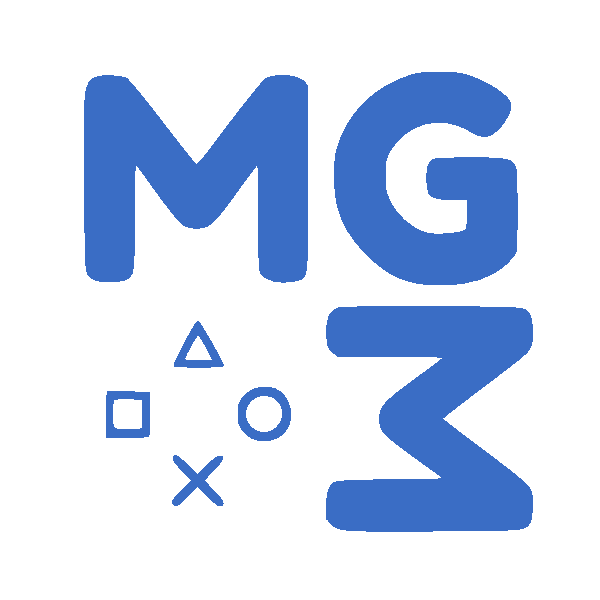
\includegraphics[height=26pt]{../proposal/assets/atlas-mark.pdf}}\hspace{8pt}%
{\bricolagexb\fontsize{34pt}{34pt}\selectfont\color{cink}Atlas}

\vspace{0.4cm}
\noindent{\bricolagesb\fontsize{16pt}{20pt}\selectfont\color{cink2} Galeri Tangkapan Layar Lengkap}

\vspace{0.3cm}
\noindent{\fontsize{10.5pt}{15pt}\selectfont\color{cink3} Dokumen pendukung teknis untuk proposal HOLOGY 9.0 HoloDev, tim MGM Unjuk Diri Dulu. Berisi 79 tangkapan layar dari instans produksi Atlas (\url{https://atlas.creations.ren}), diambil langsung dari aplikasi yang berjalan, bukan mockup. Dua puluh empat hingga dua puluh delapan tangkapan layar terbaik sudah dikurasi dan ditampilkan langsung di dalam proposal utama; dokumen ini melengkapi dengan cakupan penuh seluruh modul untuk keperluan verifikasi teknis oleh dewan juri.}

\vspace{0.5cm}
\noindent\textcolor{cline}{\rule{\linewidth}{0.8pt}}

\clearpage
\subsection*{Autentikasi dan Landing}
\vspace{0.3em}
\noindent
\begin{minipage}[t]{0.315\linewidth}
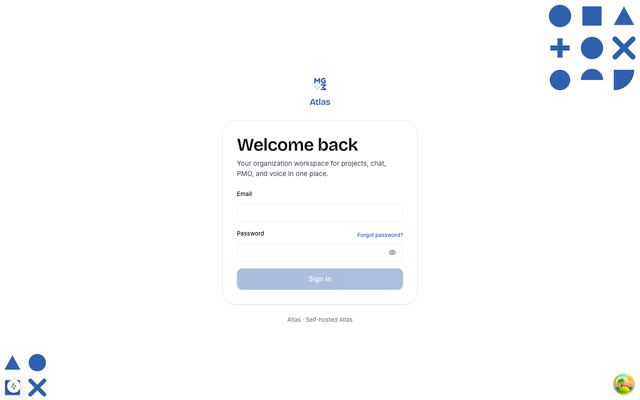
\includegraphics[width=\linewidth]{screenshots/thumbs/001-auth-landing.jpg}\\[0.15em]
{\ttfamily\scriptsize\color{cink3} 001 \quad landing}
\end{minipage}
\hfill
\begin{minipage}[t]{0.315\linewidth}
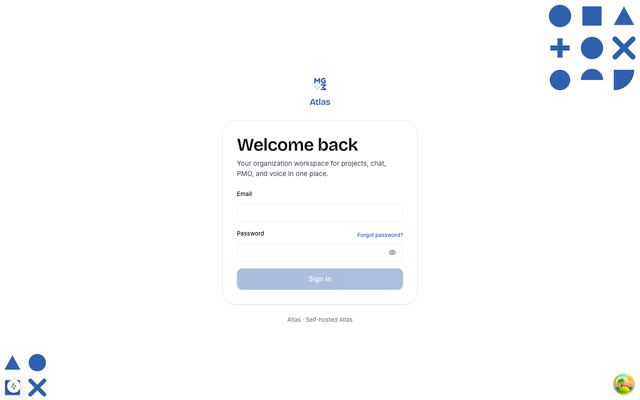
\includegraphics[width=\linewidth]{screenshots/thumbs/002-auth-login.jpg}\\[0.15em]
{\ttfamily\scriptsize\color{cink3} 002 \quad login}
\end{minipage}
\hfill
\begin{minipage}[t]{0.315\linewidth}
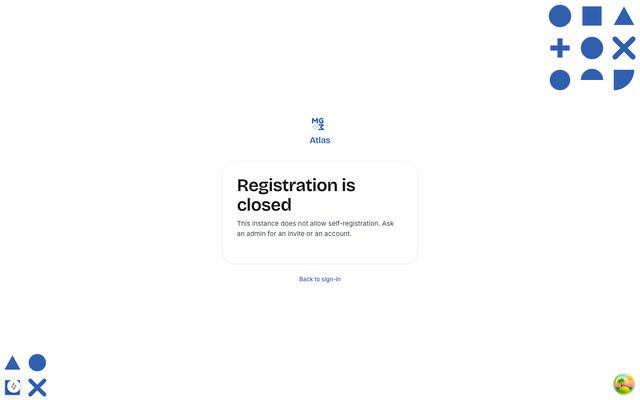
\includegraphics[width=\linewidth]{screenshots/thumbs/003-auth-register.jpg}\\[0.15em]
{\ttfamily\scriptsize\color{cink3} 003 \quad register}
\end{minipage}
\par\vspace{0.9em}
\noindent
\begin{minipage}[t]{0.315\linewidth}
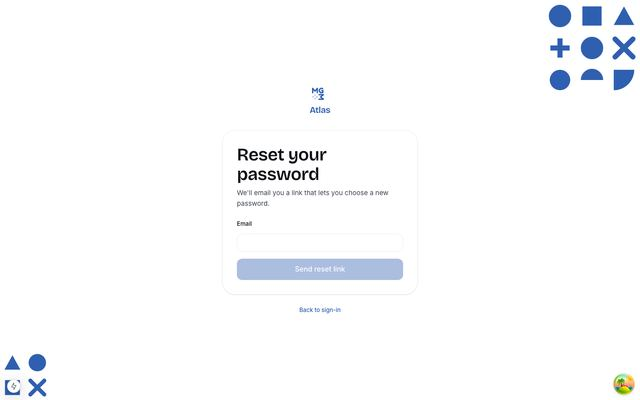
\includegraphics[width=\linewidth]{screenshots/thumbs/004-auth-forgot-password.jpg}\\[0.15em]
{\ttfamily\scriptsize\color{cink3} 004 \quad forgot password}
\end{minipage}
\hfill
\begin{minipage}[t]{0.315\linewidth}
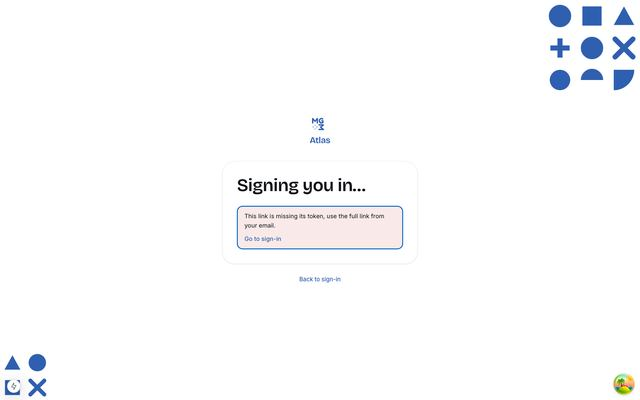
\includegraphics[width=\linewidth]{screenshots/thumbs/005-auth-magic-link.jpg}\\[0.15em]
{\ttfamily\scriptsize\color{cink3} 005 \quad magic link}
\end{minipage}

\clearpage
\subsection*{Dashboard, For Me, Notifikasi}
\vspace{0.3em}
\noindent
\begin{minipage}[t]{0.315\linewidth}
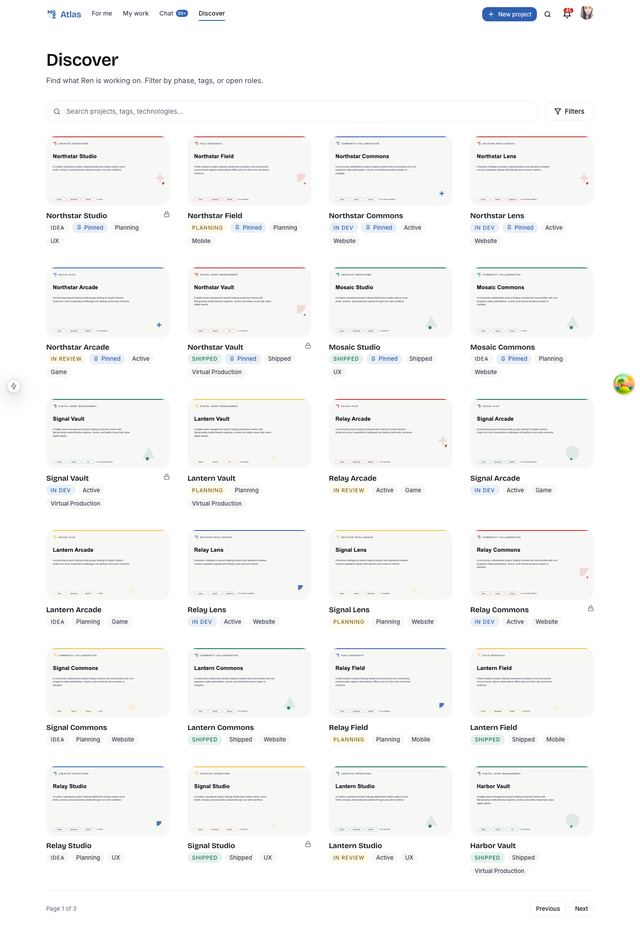
\includegraphics[width=\linewidth]{screenshots/thumbs/006-core-dashboard.jpg}\\[0.15em]
{\ttfamily\scriptsize\color{cink3} 006 \quad dashboard}
\end{minipage}
\hfill
\begin{minipage}[t]{0.315\linewidth}
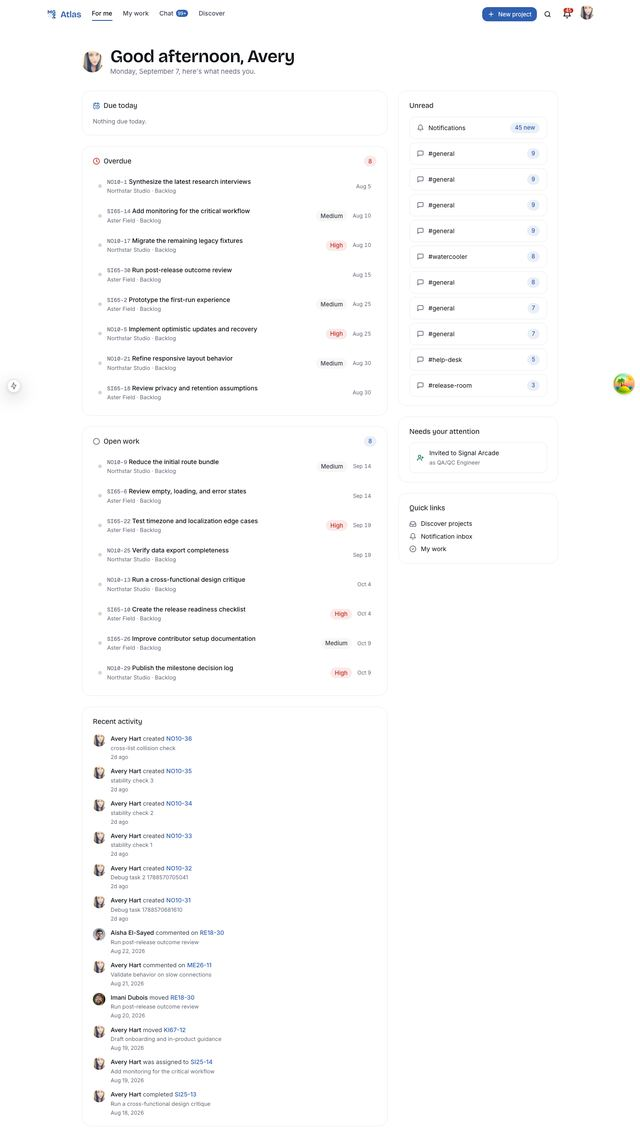
\includegraphics[width=\linewidth]{screenshots/thumbs/007-core-for-me.jpg}\\[0.15em]
{\ttfamily\scriptsize\color{cink3} 007 \quad for me}
\end{minipage}
\hfill
\begin{minipage}[t]{0.315\linewidth}
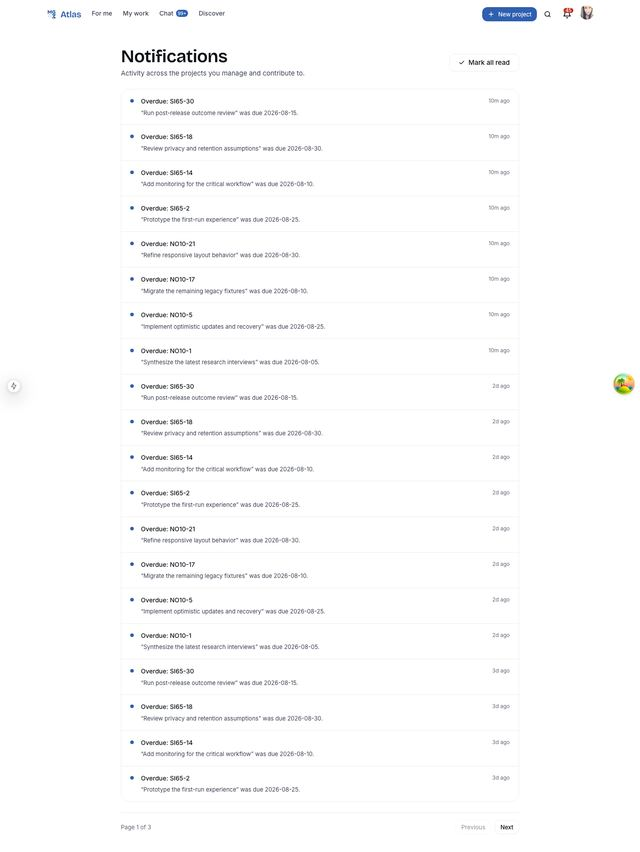
\includegraphics[width=\linewidth]{screenshots/thumbs/008-core-notifications.jpg}\\[0.15em]
{\ttfamily\scriptsize\color{cink3} 008 \quad notifications}
\end{minipage}
\par\vspace{0.9em}
\noindent
\begin{minipage}[t]{0.315\linewidth}
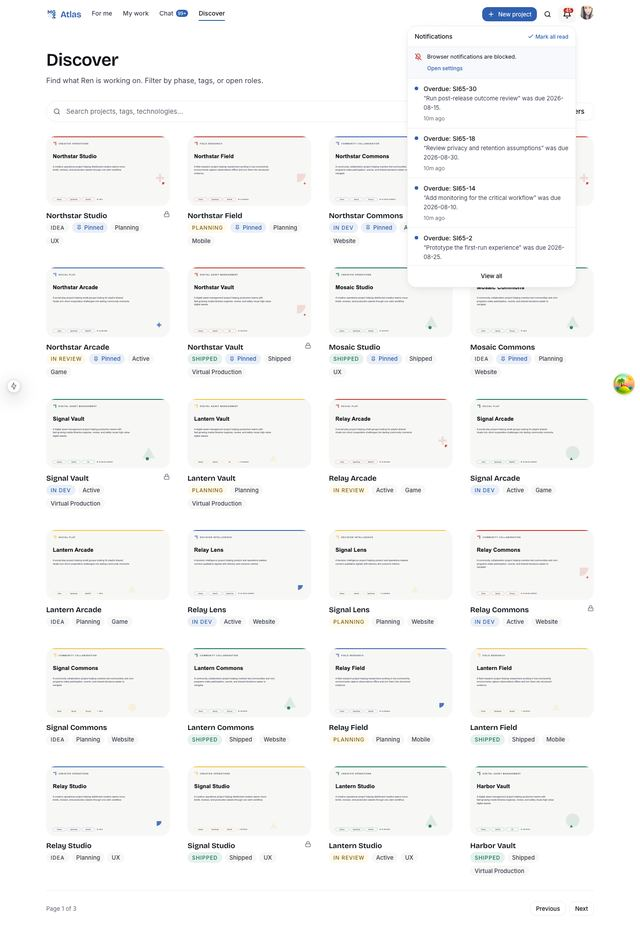
\includegraphics[width=\linewidth]{screenshots/thumbs/009-core-notif-bell-open.jpg}\\[0.15em]
{\ttfamily\scriptsize\color{cink3} 009 \quad notif bell open}
\end{minipage}
\hfill
\begin{minipage}[t]{0.315\linewidth}
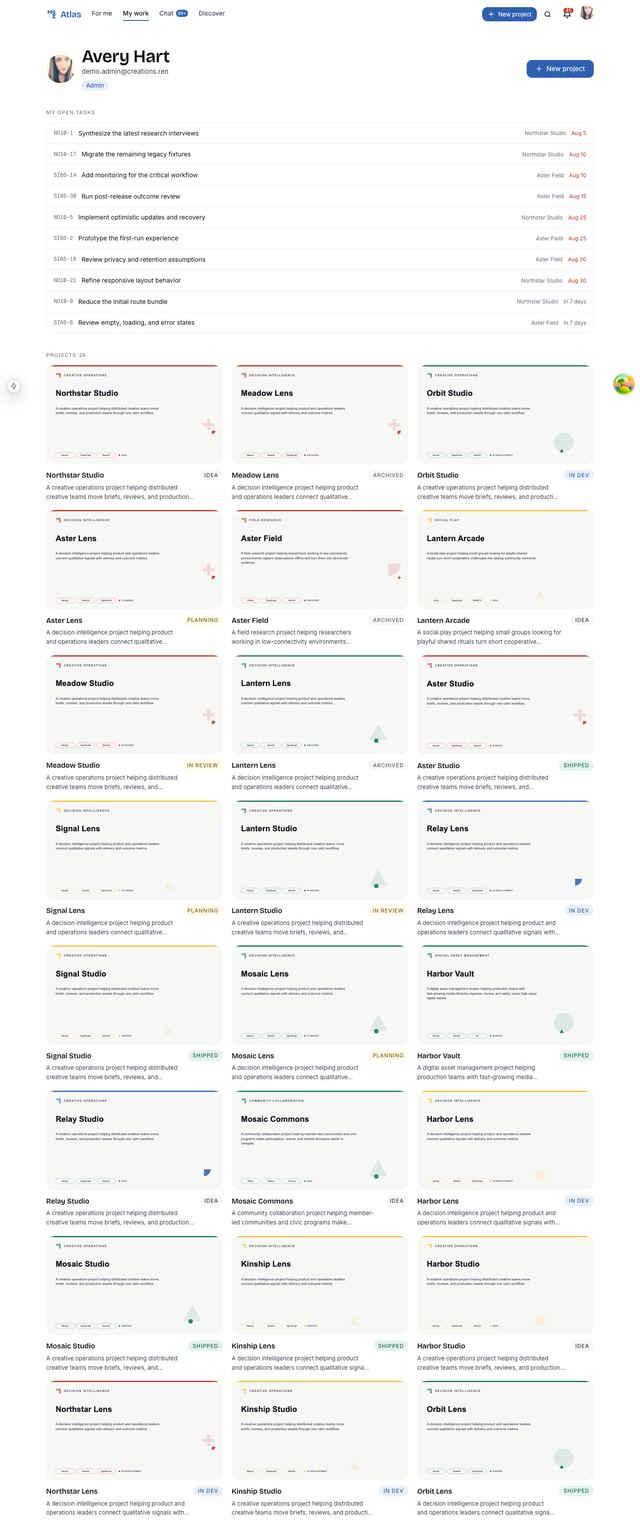
\includegraphics[width=\linewidth]{screenshots/thumbs/010-core-my-profile.jpg}\\[0.15em]
{\ttfamily\scriptsize\color{cink3} 010 \quad my profile}
\end{minipage}
\hfill
\begin{minipage}[t]{0.315\linewidth}
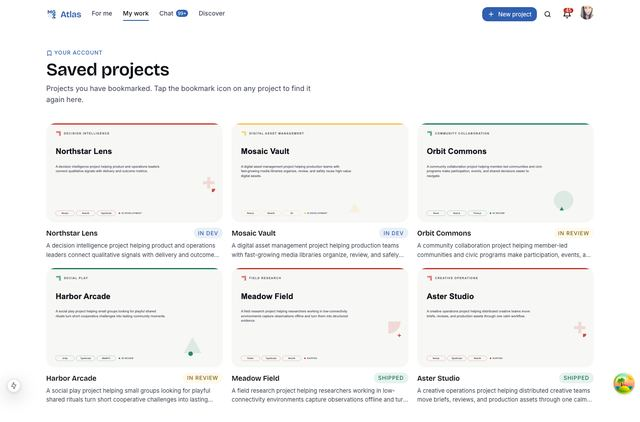
\includegraphics[width=\linewidth]{screenshots/thumbs/011-core-saved.jpg}\\[0.15em]
{\ttfamily\scriptsize\color{cink3} 011 \quad saved}
\end{minipage}

\clearpage
\subsection*{Manajemen Proyek}
\vspace{0.3em}
\noindent
\begin{minipage}[t]{0.315\linewidth}
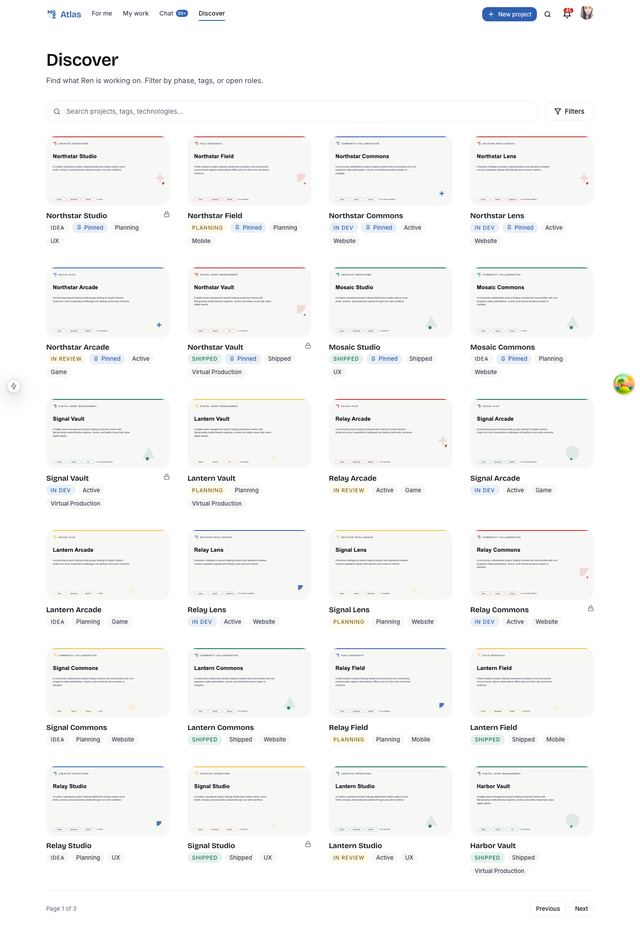
\includegraphics[width=\linewidth]{screenshots/thumbs/012-projects-grid.jpg}\\[0.15em]
{\ttfamily\scriptsize\color{cink3} 012 \quad grid}
\end{minipage}
\hfill
\begin{minipage}[t]{0.315\linewidth}
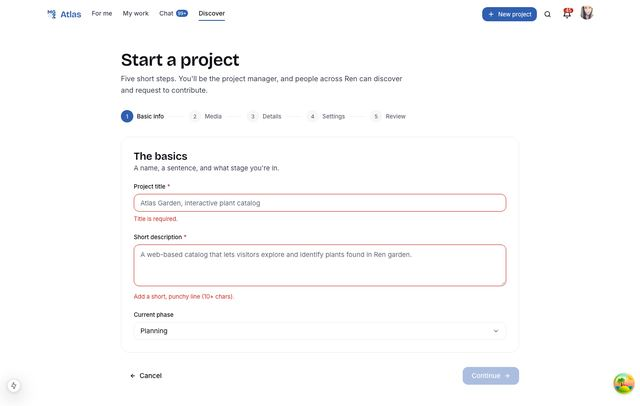
\includegraphics[width=\linewidth]{screenshots/thumbs/013-projects-new.jpg}\\[0.15em]
{\ttfamily\scriptsize\color{cink3} 013 \quad new}
\end{minipage}
\hfill
\begin{minipage}[t]{0.315\linewidth}
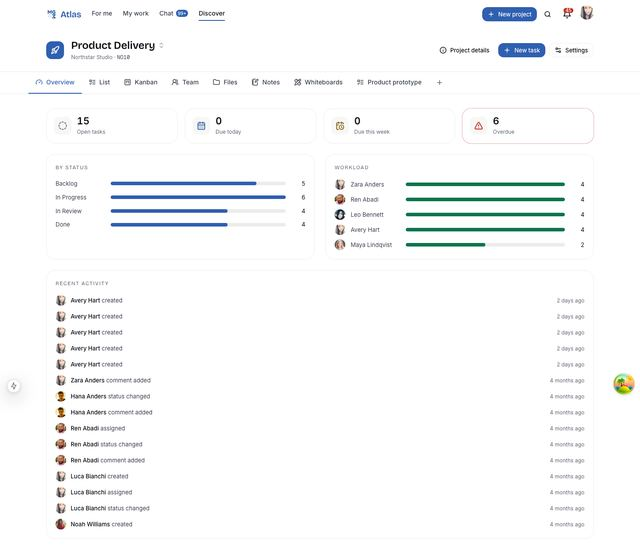
\includegraphics[width=\linewidth]{screenshots/thumbs/014-projects-overview.jpg}\\[0.15em]
{\ttfamily\scriptsize\color{cink3} 014 \quad overview}
\end{minipage}
\par\vspace{0.9em}
\noindent
\begin{minipage}[t]{0.315\linewidth}
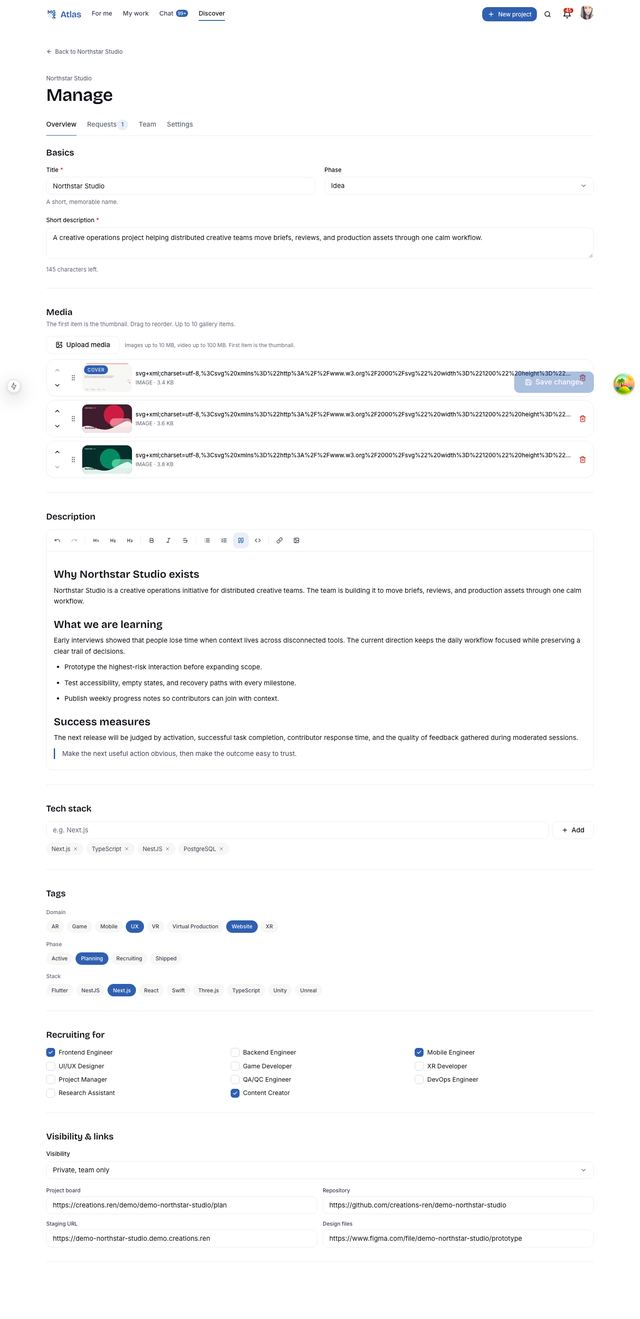
\includegraphics[width=\linewidth]{screenshots/thumbs/015-projects-manage.jpg}\\[0.15em]
{\ttfamily\scriptsize\color{cink3} 015 \quad manage}
\end{minipage}
\hfill
\begin{minipage}[t]{0.315\linewidth}
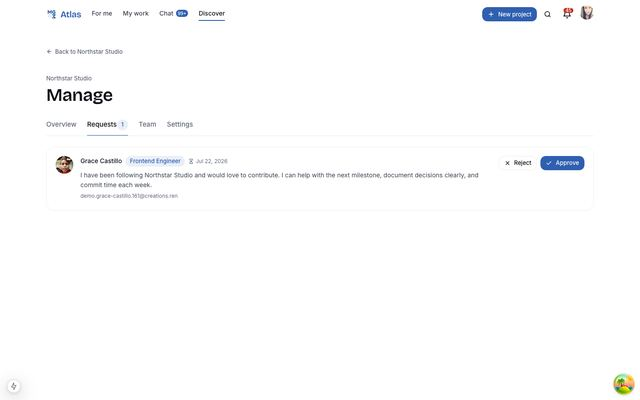
\includegraphics[width=\linewidth]{screenshots/thumbs/016-projects-manage-requests.jpg}\\[0.15em]
{\ttfamily\scriptsize\color{cink3} 016 \quad manage requests}
\end{minipage}
\hfill
\begin{minipage}[t]{0.315\linewidth}
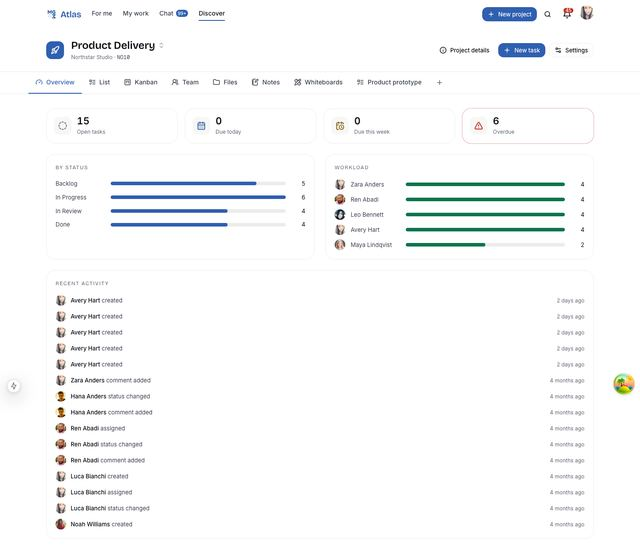
\includegraphics[width=\linewidth]{screenshots/thumbs/017-projects-lists.jpg}\\[0.15em]
{\ttfamily\scriptsize\color{cink3} 017 \quad lists}
\end{minipage}
\par\vspace{0.9em}
\noindent
\begin{minipage}[t]{0.315\linewidth}
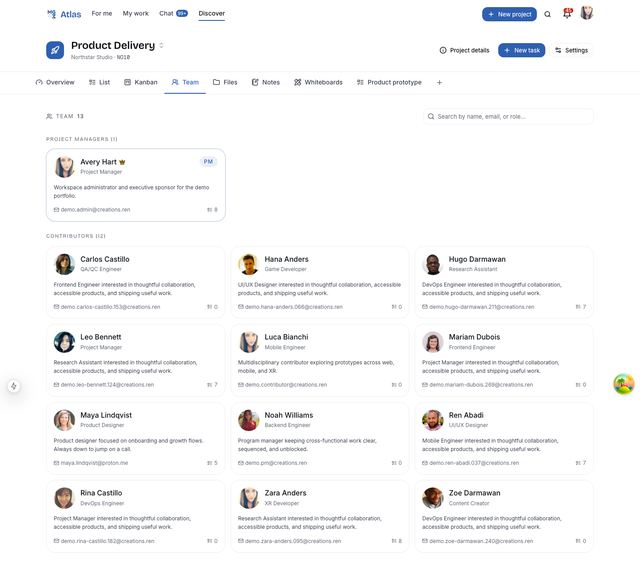
\includegraphics[width=\linewidth]{screenshots/thumbs/018-projects-team.jpg}\\[0.15em]
{\ttfamily\scriptsize\color{cink3} 018 \quad team}
\end{minipage}

\clearpage
\subsection*{PMO: Kanban, List, Timeline, Catatan, Whiteboard}
\vspace{0.3em}
\noindent
\begin{minipage}[t]{0.315\linewidth}
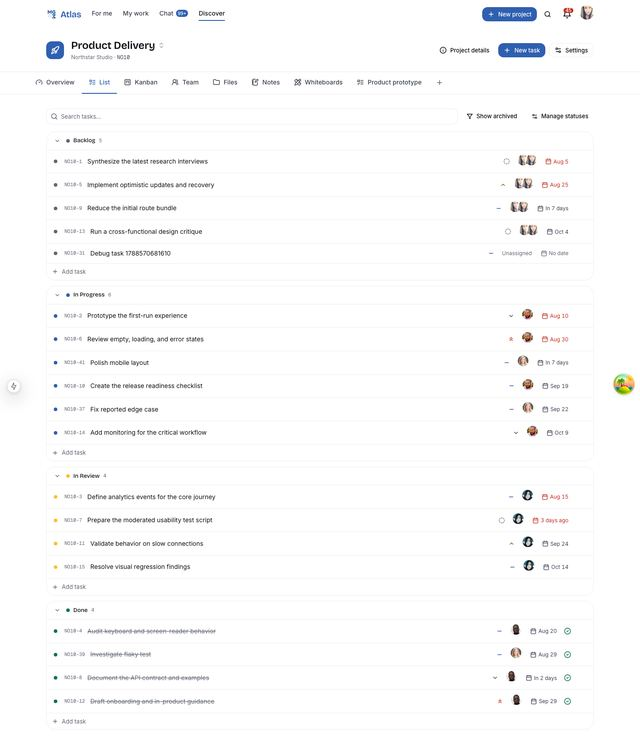
\includegraphics[width=\linewidth]{screenshots/thumbs/019-pmo-list-view.jpg}\\[0.15em]
{\ttfamily\scriptsize\color{cink3} 019 \quad list view}
\end{minipage}
\hfill
\begin{minipage}[t]{0.315\linewidth}
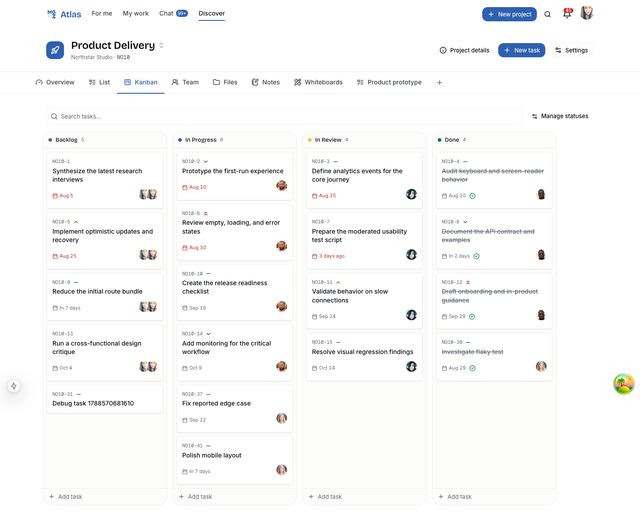
\includegraphics[width=\linewidth]{screenshots/thumbs/020-pmo-kanban.jpg}\\[0.15em]
{\ttfamily\scriptsize\color{cink3} 020 \quad kanban}
\end{minipage}
\hfill
\begin{minipage}[t]{0.315\linewidth}
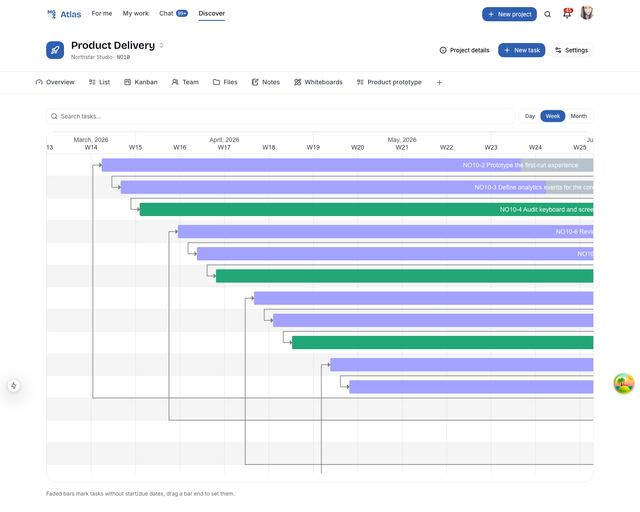
\includegraphics[width=\linewidth]{screenshots/thumbs/021-pmo-timeline.jpg}\\[0.15em]
{\ttfamily\scriptsize\color{cink3} 021 \quad timeline}
\end{minipage}
\par\vspace{0.9em}
\noindent
\begin{minipage}[t]{0.315\linewidth}
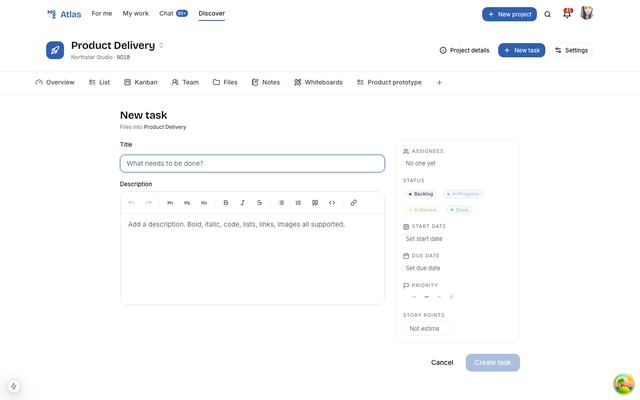
\includegraphics[width=\linewidth]{screenshots/thumbs/022-pmo-task-new.jpg}\\[0.15em]
{\ttfamily\scriptsize\color{cink3} 022 \quad task new}
\end{minipage}
\hfill
\begin{minipage}[t]{0.315\linewidth}
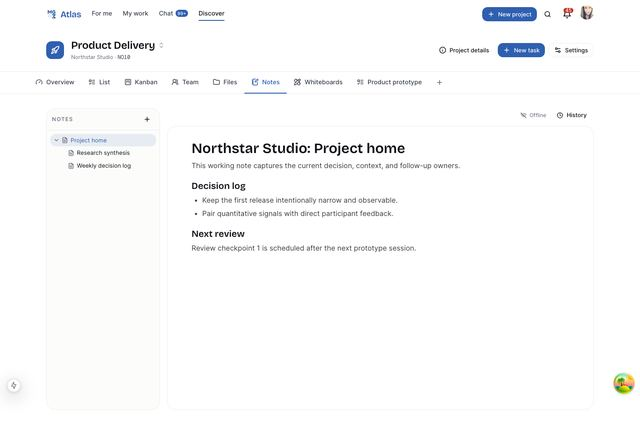
\includegraphics[width=\linewidth]{screenshots/thumbs/023-pmo-notes.jpg}\\[0.15em]
{\ttfamily\scriptsize\color{cink3} 023 \quad notes}
\end{minipage}
\hfill
\begin{minipage}[t]{0.315\linewidth}
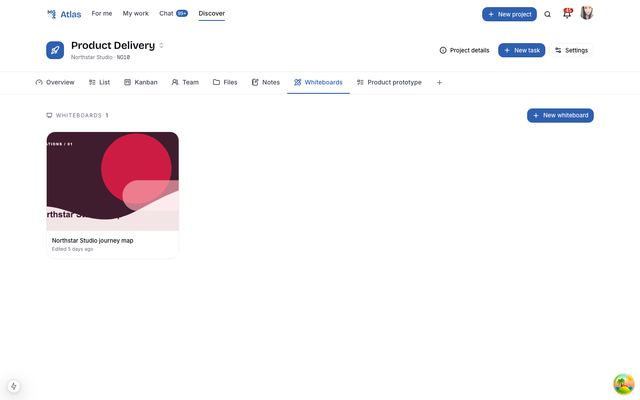
\includegraphics[width=\linewidth]{screenshots/thumbs/024-pmo-whiteboards-list.jpg}\\[0.15em]
{\ttfamily\scriptsize\color{cink3} 024 \quad whiteboards list}
\end{minipage}
\par\vspace{0.9em}
\noindent
\begin{minipage}[t]{0.315\linewidth}
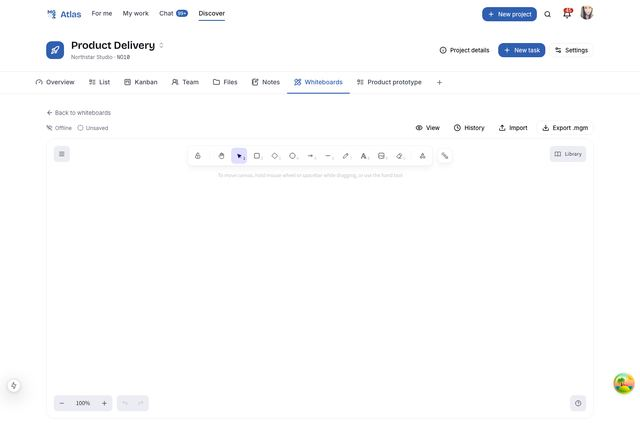
\includegraphics[width=\linewidth]{screenshots/thumbs/025-pmo-whiteboard-canvas.jpg}\\[0.15em]
{\ttfamily\scriptsize\color{cink3} 025 \quad whiteboard canvas}
\end{minipage}
\hfill
\begin{minipage}[t]{0.315\linewidth}
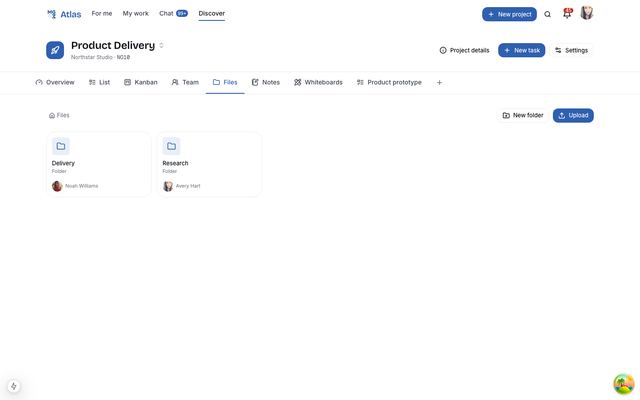
\includegraphics[width=\linewidth]{screenshots/thumbs/026-pmo-files.jpg}\\[0.15em]
{\ttfamily\scriptsize\color{cink3} 026 \quad files}
\end{minipage}
\hfill
\begin{minipage}[t]{0.315\linewidth}
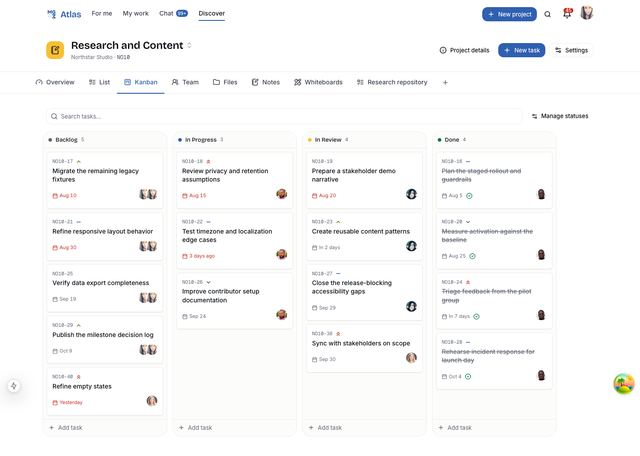
\includegraphics[width=\linewidth]{screenshots/thumbs/027-pmo-list2-kanban.jpg}\\[0.15em]
{\ttfamily\scriptsize\color{cink3} 027 \quad list2 kanban}
\end{minipage}
\par\vspace{0.9em}
\noindent
\begin{minipage}[t]{0.315\linewidth}
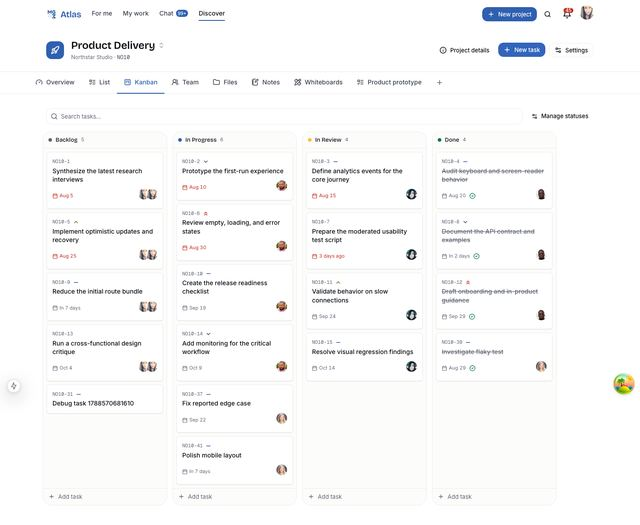
\includegraphics[width=\linewidth]{screenshots/thumbs/028-pmo-task-detail-modal.jpg}\\[0.15em]
{\ttfamily\scriptsize\color{cink3} 028 \quad task detail modal}
\end{minipage}

\clearpage
\subsection*{Obrolan Tim}
\vspace{0.3em}
\noindent
\begin{minipage}[t]{0.315\linewidth}
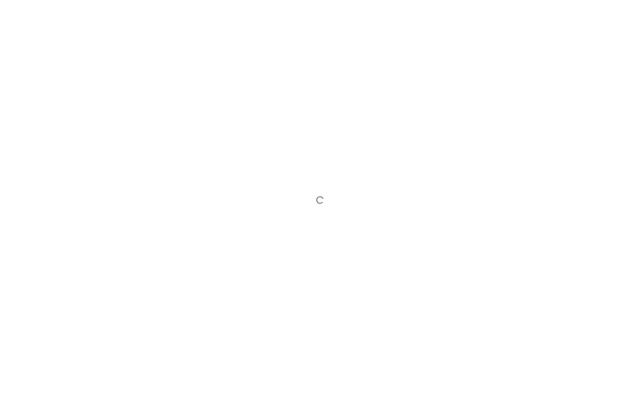
\includegraphics[width=\linewidth]{screenshots/thumbs/029-chat-global-landing.jpg}\\[0.15em]
{\ttfamily\scriptsize\color{cink3} 029 \quad global landing}
\end{minipage}
\hfill
\begin{minipage}[t]{0.315\linewidth}
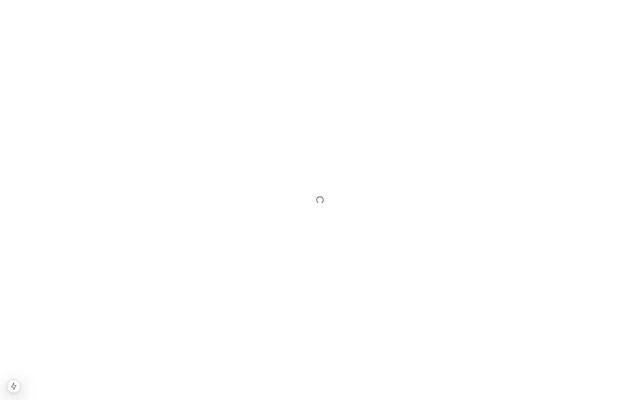
\includegraphics[width=\linewidth]{screenshots/thumbs/030-chat-global-community.jpg}\\[0.15em]
{\ttfamily\scriptsize\color{cink3} 030 \quad global community}
\end{minipage}
\hfill
\begin{minipage}[t]{0.315\linewidth}
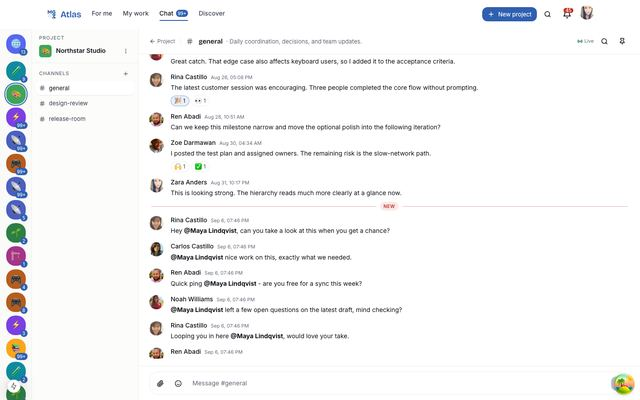
\includegraphics[width=\linewidth]{screenshots/thumbs/031-chat-project-landing.jpg}\\[0.15em]
{\ttfamily\scriptsize\color{cink3} 031 \quad project landing}
\end{minipage}
\par\vspace{0.9em}
\noindent
\begin{minipage}[t]{0.315\linewidth}
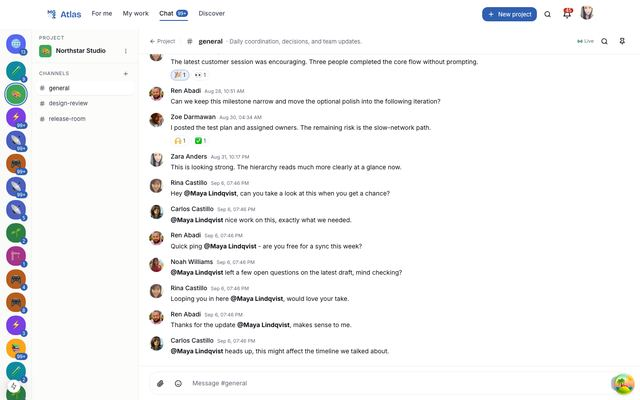
\includegraphics[width=\linewidth]{screenshots/thumbs/032-chat-project-general.jpg}\\[0.15em]
{\ttfamily\scriptsize\color{cink3} 032 \quad project general}
\end{minipage}
\hfill
\begin{minipage}[t]{0.315\linewidth}
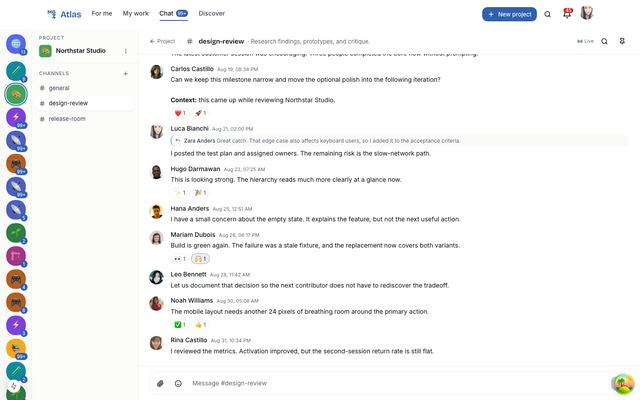
\includegraphics[width=\linewidth]{screenshots/thumbs/033-chat-project-design-review.jpg}\\[0.15em]
{\ttfamily\scriptsize\color{cink3} 033 \quad project design review}
\end{minipage}
\hfill
\begin{minipage}[t]{0.315\linewidth}
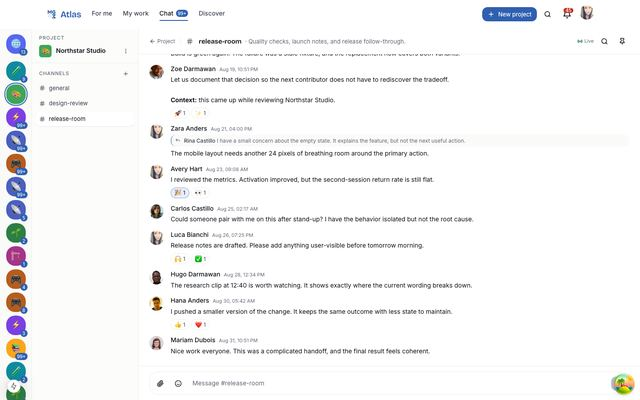
\includegraphics[width=\linewidth]{screenshots/thumbs/034-chat-project-release-room.jpg}\\[0.15em]
{\ttfamily\scriptsize\color{cink3} 034 \quad project release room}
\end{minipage}

\clearpage
\subsection*{Panggilan Suara}
\vspace{0.3em}
\noindent
\begin{minipage}[t]{0.315\linewidth}
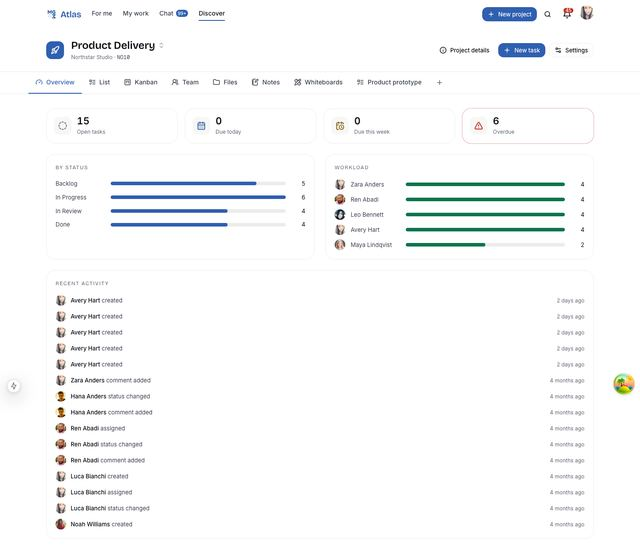
\includegraphics[width=\linewidth]{screenshots/thumbs/035-voice-project-sidebar-entry.jpg}\\[0.15em]
{\ttfamily\scriptsize\color{cink3} 035 \quad project sidebar entry}
\end{minipage}

\clearpage
\subsection*{Godmode: Panel Kendali Swa-hosting}
\vspace{0.3em}
\noindent
\begin{minipage}[t]{0.315\linewidth}
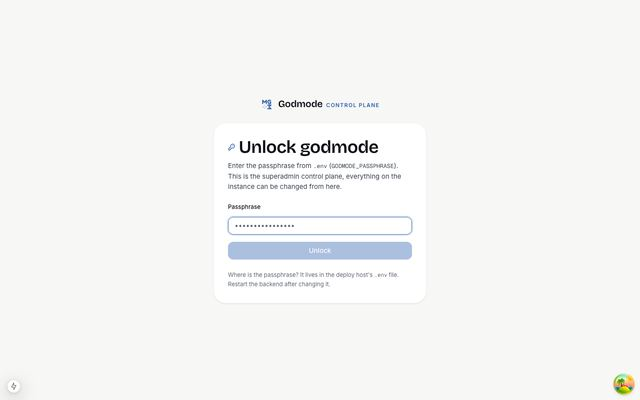
\includegraphics[width=\linewidth]{screenshots/thumbs/036-godmode-unlock-screen.jpg}\\[0.15em]
{\ttfamily\scriptsize\color{cink3} 036 \quad unlock screen}
\end{minipage}
\hfill
\begin{minipage}[t]{0.315\linewidth}
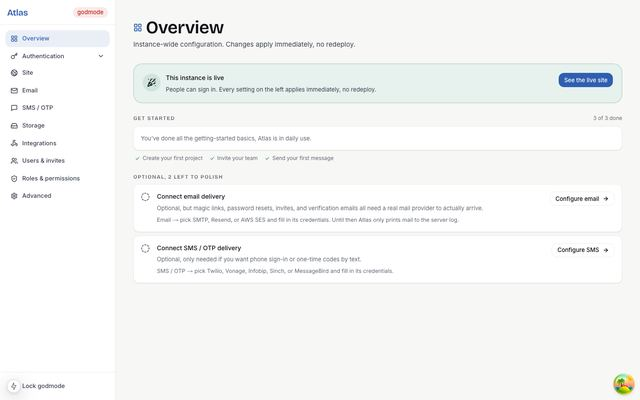
\includegraphics[width=\linewidth]{screenshots/thumbs/037-godmode-overview.jpg}\\[0.15em]
{\ttfamily\scriptsize\color{cink3} 037 \quad overview}
\end{minipage}
\hfill
\begin{minipage}[t]{0.315\linewidth}
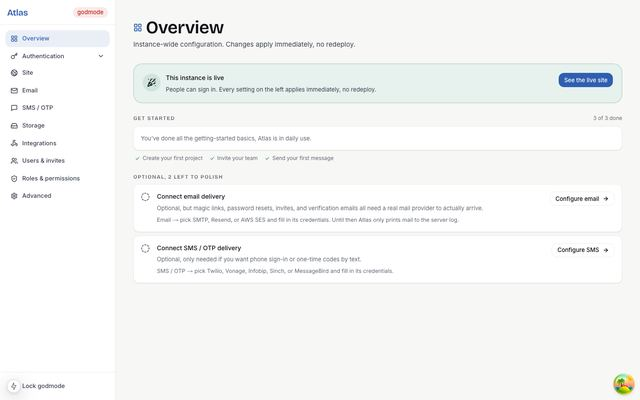
\includegraphics[width=\linewidth]{screenshots/thumbs/038-godmode-users.jpg}\\[0.15em]
{\ttfamily\scriptsize\color{cink3} 038 \quad users}
\end{minipage}
\par\vspace{0.9em}
\noindent
\begin{minipage}[t]{0.315\linewidth}
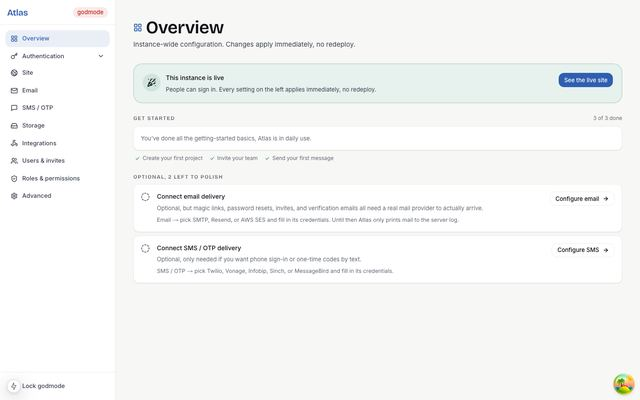
\includegraphics[width=\linewidth]{screenshots/thumbs/039-godmode-roles.jpg}\\[0.15em]
{\ttfamily\scriptsize\color{cink3} 039 \quad roles}
\end{minipage}
\hfill
\begin{minipage}[t]{0.315\linewidth}
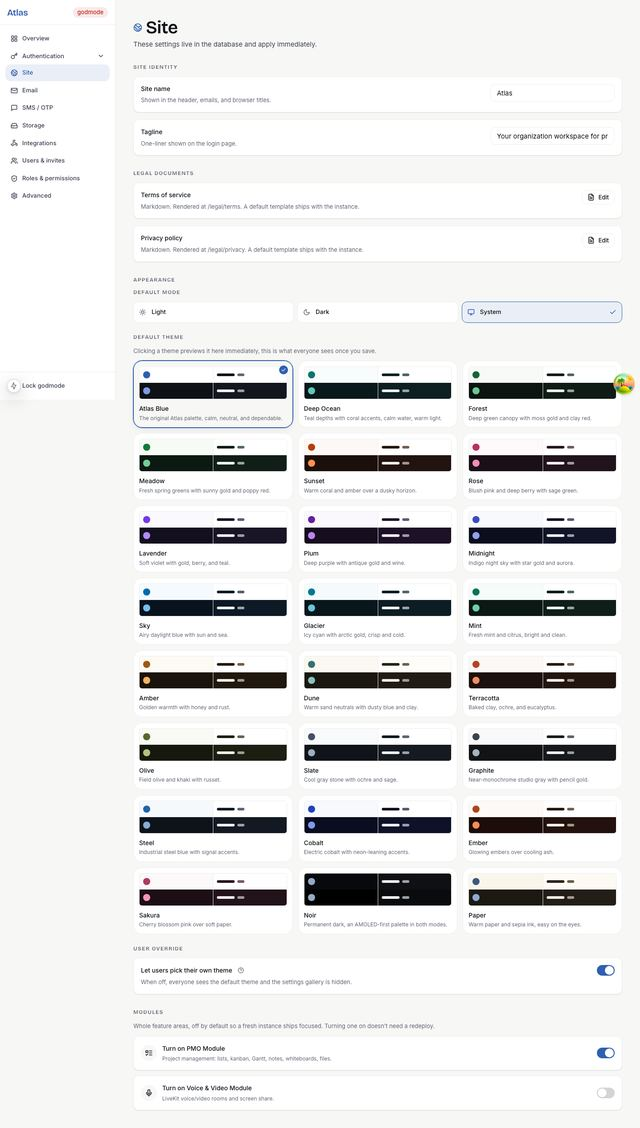
\includegraphics[width=\linewidth]{screenshots/thumbs/040-godmode-site.jpg}\\[0.15em]
{\ttfamily\scriptsize\color{cink3} 040 \quad site}
\end{minipage}
\hfill
\begin{minipage}[t]{0.315\linewidth}
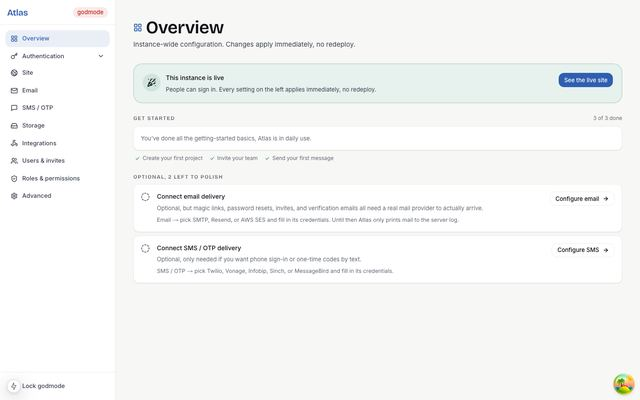
\includegraphics[width=\linewidth]{screenshots/thumbs/041-godmode-appearance.jpg}\\[0.15em]
{\ttfamily\scriptsize\color{cink3} 041 \quad appearance}
\end{minipage}
\par\vspace{0.9em}
\noindent
\begin{minipage}[t]{0.315\linewidth}
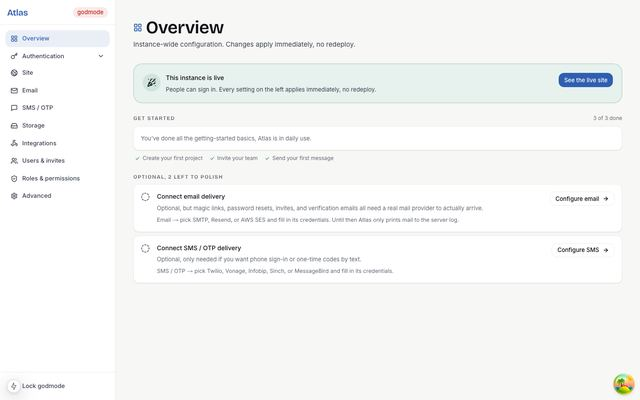
\includegraphics[width=\linewidth]{screenshots/thumbs/042-godmode-registration.jpg}\\[0.15em]
{\ttfamily\scriptsize\color{cink3} 042 \quad registration}
\end{minipage}
\hfill
\begin{minipage}[t]{0.315\linewidth}
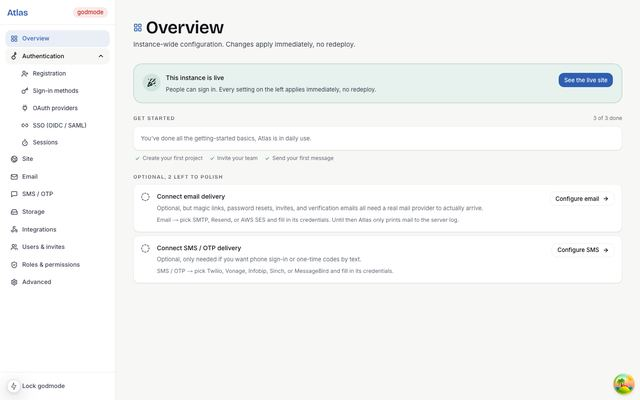
\includegraphics[width=\linewidth]{screenshots/thumbs/043-godmode-authentication.jpg}\\[0.15em]
{\ttfamily\scriptsize\color{cink3} 043 \quad authentication}
\end{minipage}
\hfill
\begin{minipage}[t]{0.315\linewidth}
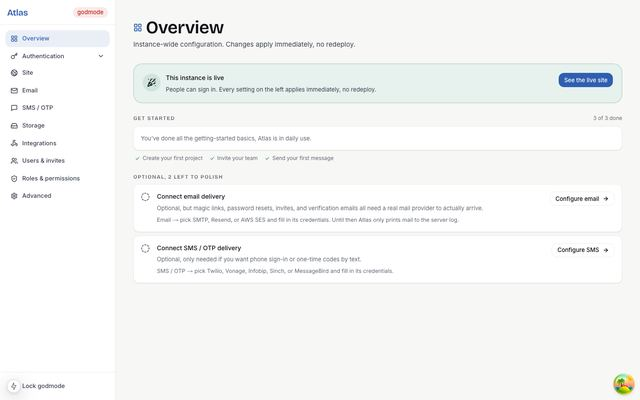
\includegraphics[width=\linewidth]{screenshots/thumbs/044-godmode-sessions-policy.jpg}\\[0.15em]
{\ttfamily\scriptsize\color{cink3} 044 \quad sessions policy}
\end{minipage}
\par\vspace{0.9em}
\noindent
\begin{minipage}[t]{0.315\linewidth}
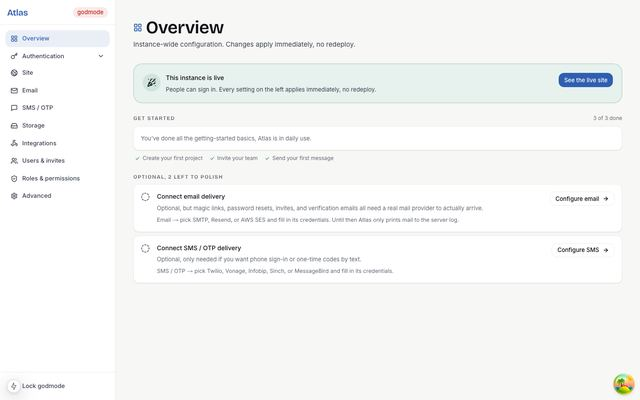
\includegraphics[width=\linewidth]{screenshots/thumbs/045-godmode-oauth.jpg}\\[0.15em]
{\ttfamily\scriptsize\color{cink3} 045 \quad oauth}
\end{minipage}
\hfill
\begin{minipage}[t]{0.315\linewidth}
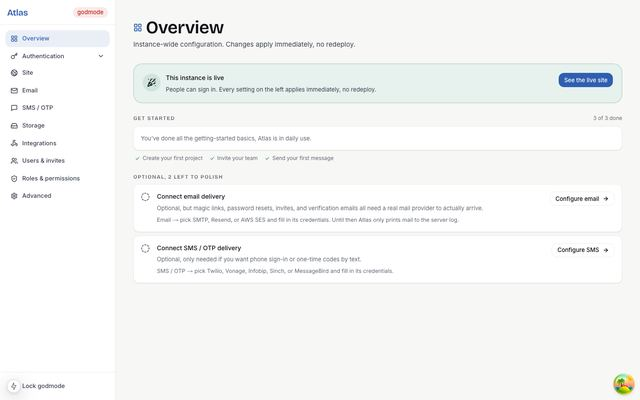
\includegraphics[width=\linewidth]{screenshots/thumbs/046-godmode-sso.jpg}\\[0.15em]
{\ttfamily\scriptsize\color{cink3} 046 \quad sso}
\end{minipage}
\hfill
\begin{minipage}[t]{0.315\linewidth}
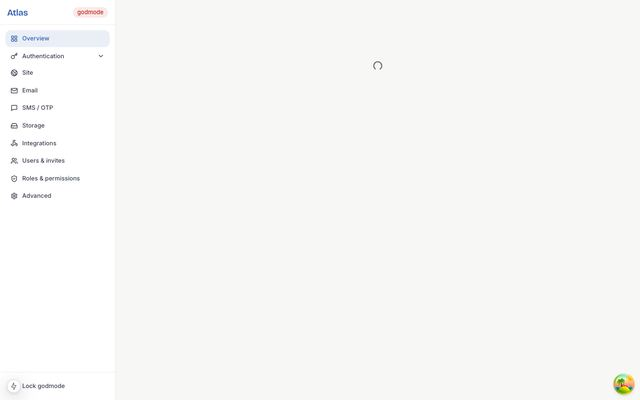
\includegraphics[width=\linewidth]{screenshots/thumbs/047-godmode-storage.jpg}\\[0.15em]
{\ttfamily\scriptsize\color{cink3} 047 \quad storage}
\end{minipage}
\par\vspace{0.9em}
\noindent
\begin{minipage}[t]{0.315\linewidth}
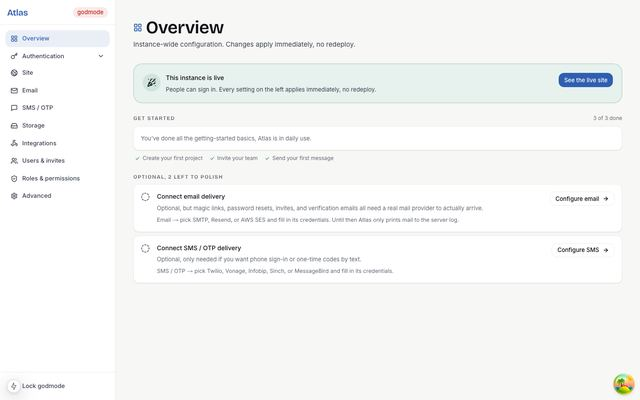
\includegraphics[width=\linewidth]{screenshots/thumbs/048-godmode-modules.jpg}\\[0.15em]
{\ttfamily\scriptsize\color{cink3} 048 \quad modules}
\end{minipage}
\hfill
\begin{minipage}[t]{0.315\linewidth}
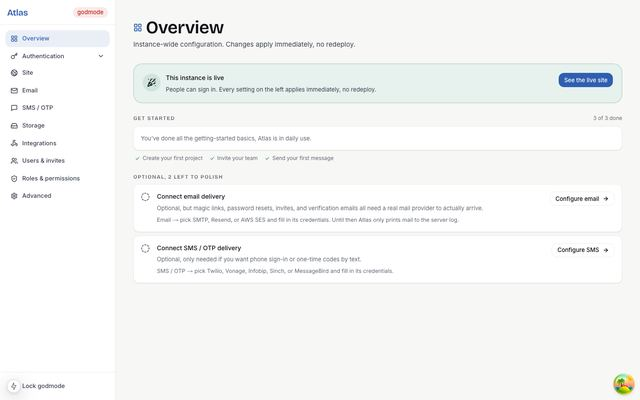
\includegraphics[width=\linewidth]{screenshots/thumbs/049-godmode-legal.jpg}\\[0.15em]
{\ttfamily\scriptsize\color{cink3} 049 \quad legal}
\end{minipage}

\clearpage
\subsection*{Konsol Admin}
\vspace{0.3em}
\noindent
\begin{minipage}[t]{0.315\linewidth}
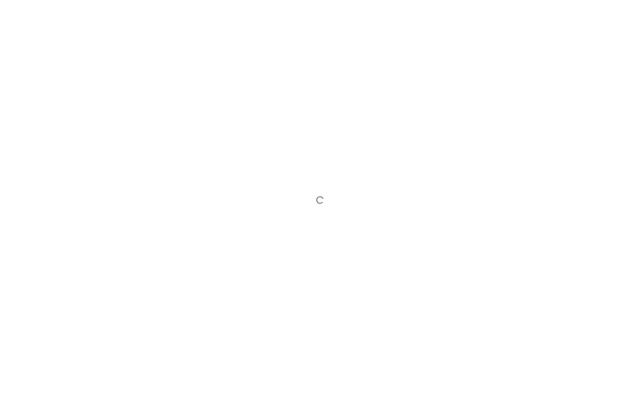
\includegraphics[width=\linewidth]{screenshots/thumbs/050-admin-tags.jpg}\\[0.15em]
{\ttfamily\scriptsize\color{cink3} 050 \quad tags}
\end{minipage}
\hfill
\begin{minipage}[t]{0.315\linewidth}
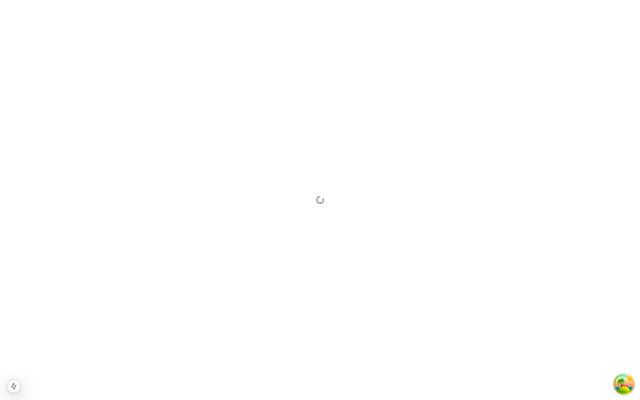
\includegraphics[width=\linewidth]{screenshots/thumbs/051-admin-featured.jpg}\\[0.15em]
{\ttfamily\scriptsize\color{cink3} 051 \quad featured}
\end{minipage}
\hfill
\begin{minipage}[t]{0.315\linewidth}
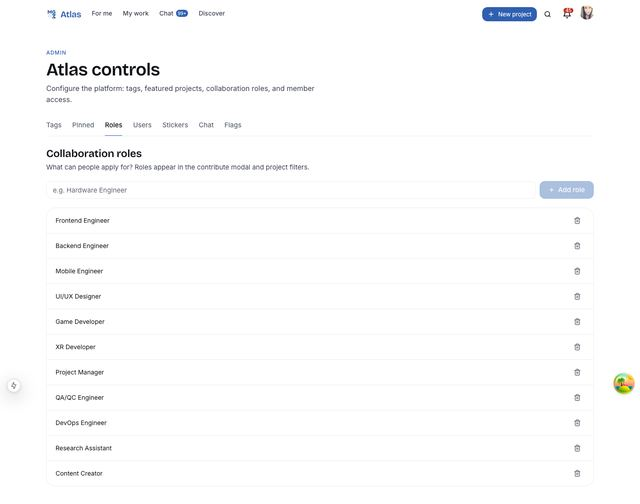
\includegraphics[width=\linewidth]{screenshots/thumbs/052-admin-roles.jpg}\\[0.15em]
{\ttfamily\scriptsize\color{cink3} 052 \quad roles}
\end{minipage}
\par\vspace{0.9em}
\noindent
\begin{minipage}[t]{0.315\linewidth}
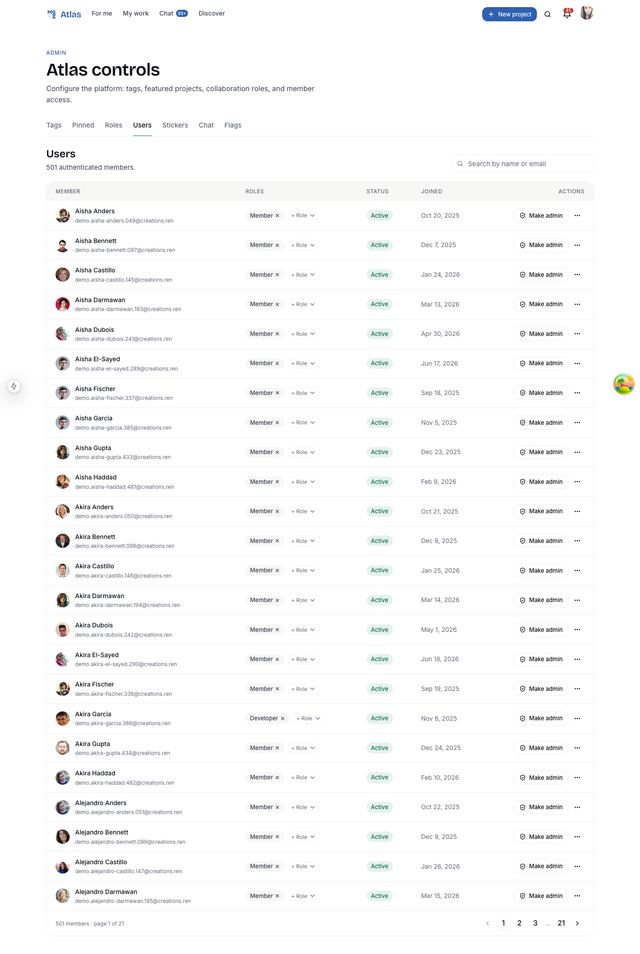
\includegraphics[width=\linewidth]{screenshots/thumbs/053-admin-users.jpg}\\[0.15em]
{\ttfamily\scriptsize\color{cink3} 053 \quad users}
\end{minipage}
\hfill
\begin{minipage}[t]{0.315\linewidth}
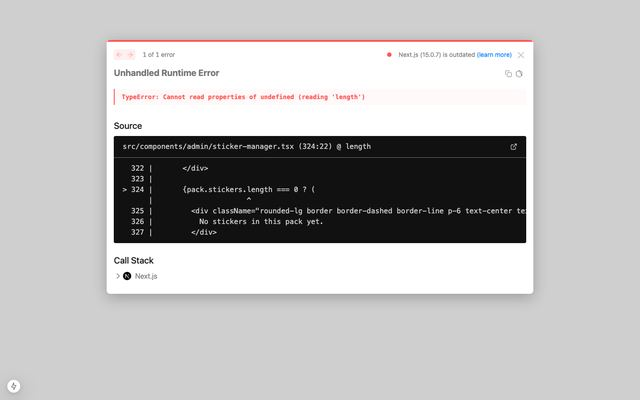
\includegraphics[width=\linewidth]{screenshots/thumbs/054-admin-stickers.jpg}\\[0.15em]
{\ttfamily\scriptsize\color{cink3} 054 \quad stickers}
\end{minipage}
\hfill
\begin{minipage}[t]{0.315\linewidth}
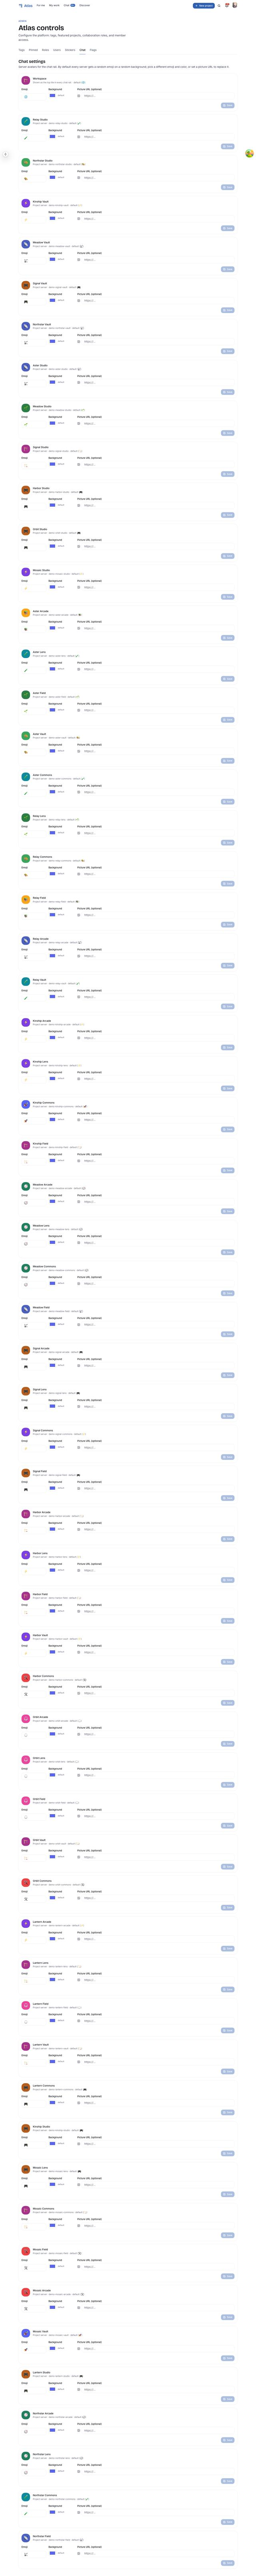
\includegraphics[width=\linewidth]{screenshots/thumbs/055-admin-chat.jpg}\\[0.15em]
{\ttfamily\scriptsize\color{cink3} 055 \quad chat}
\end{minipage}
\par\vspace{0.9em}
\noindent
\begin{minipage}[t]{0.315\linewidth}
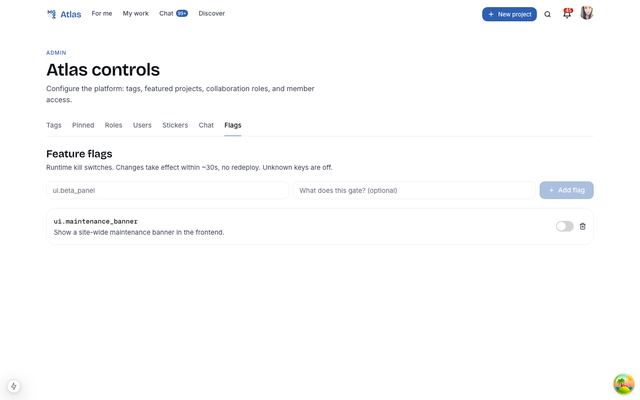
\includegraphics[width=\linewidth]{screenshots/thumbs/056-admin-flags.jpg}\\[0.15em]
{\ttfamily\scriptsize\color{cink3} 056 \quad flags}
\end{minipage}

\clearpage
\subsection*{Pengaturan Personal}
\vspace{0.3em}
\noindent
\begin{minipage}[t]{0.315\linewidth}
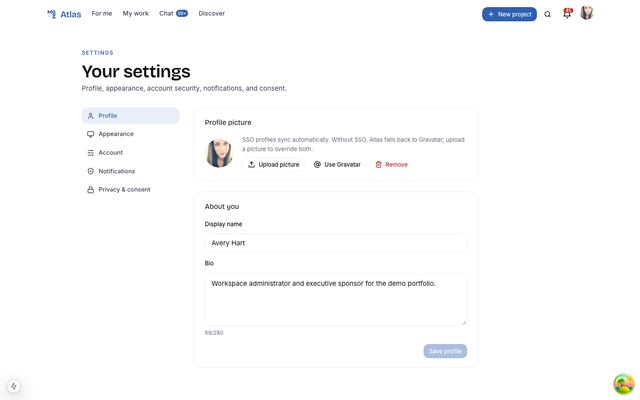
\includegraphics[width=\linewidth]{screenshots/thumbs/057-settings-hub.jpg}\\[0.15em]
{\ttfamily\scriptsize\color{cink3} 057 \quad hub}
\end{minipage}
\hfill
\begin{minipage}[t]{0.315\linewidth}
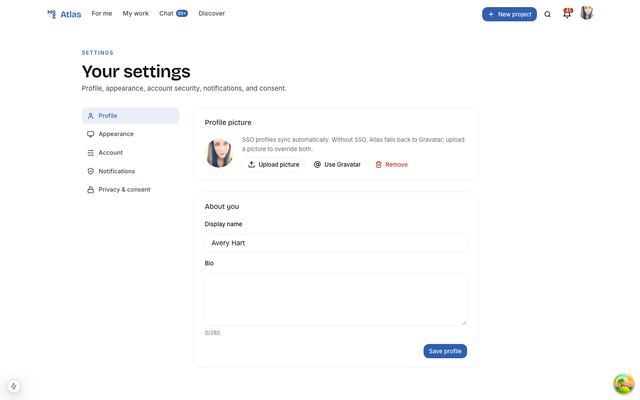
\includegraphics[width=\linewidth]{screenshots/thumbs/058-settings-profile.jpg}\\[0.15em]
{\ttfamily\scriptsize\color{cink3} 058 \quad profile}
\end{minipage}
\hfill
\begin{minipage}[t]{0.315\linewidth}
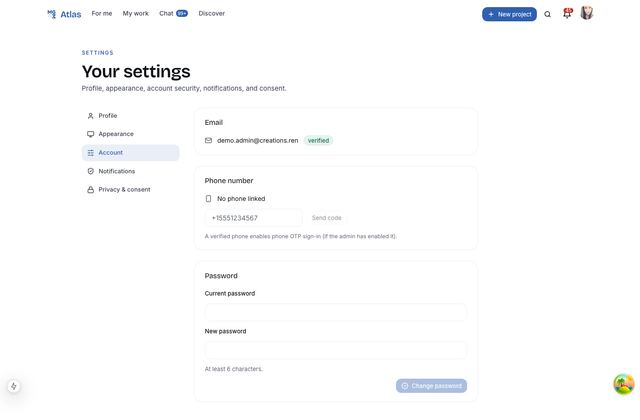
\includegraphics[width=\linewidth]{screenshots/thumbs/059-settings-account.jpg}\\[0.15em]
{\ttfamily\scriptsize\color{cink3} 059 \quad account}
\end{minipage}
\par\vspace{0.9em}
\noindent
\begin{minipage}[t]{0.315\linewidth}
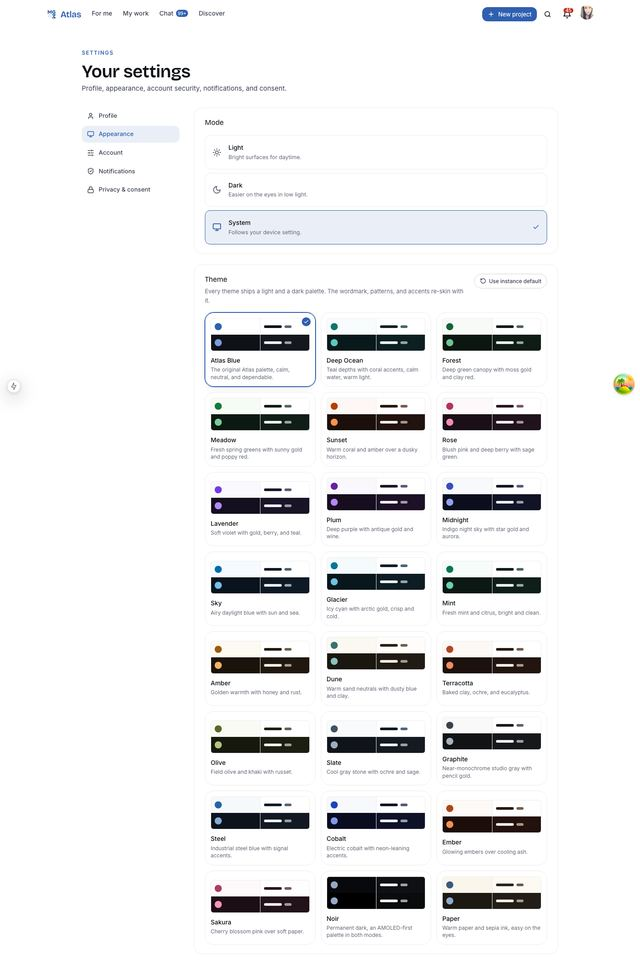
\includegraphics[width=\linewidth]{screenshots/thumbs/060-settings-appearance.jpg}\\[0.15em]
{\ttfamily\scriptsize\color{cink3} 060 \quad appearance}
\end{minipage}
\hfill
\begin{minipage}[t]{0.315\linewidth}
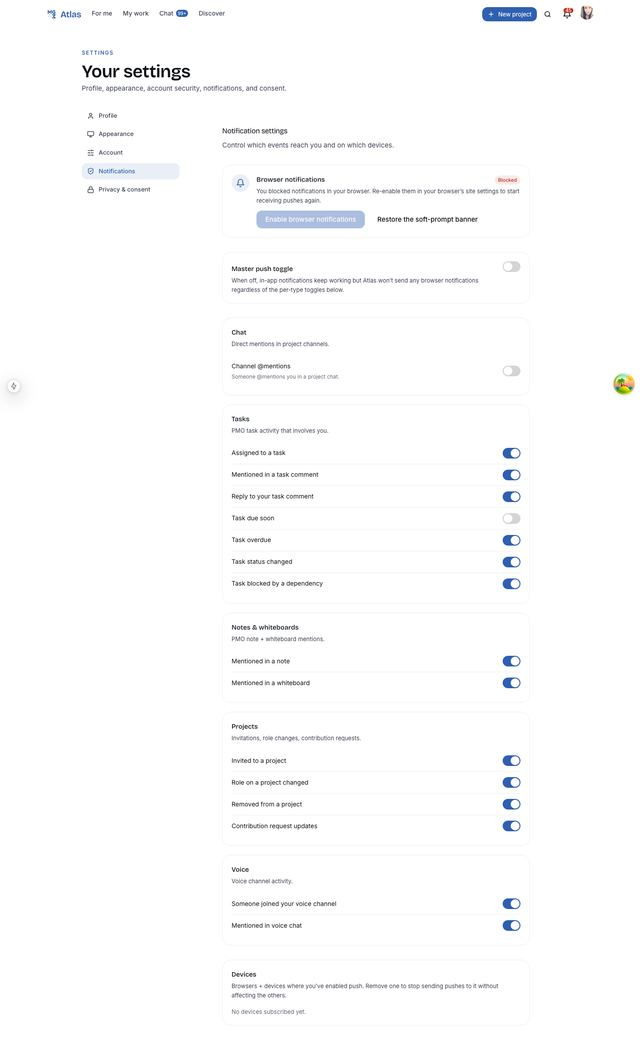
\includegraphics[width=\linewidth]{screenshots/thumbs/061-settings-notifications.jpg}\\[0.15em]
{\ttfamily\scriptsize\color{cink3} 061 \quad notifications}
\end{minipage}
\hfill
\begin{minipage}[t]{0.315\linewidth}
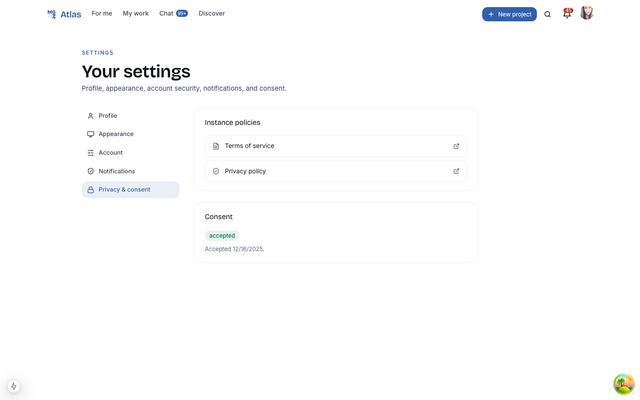
\includegraphics[width=\linewidth]{screenshots/thumbs/062-settings-privacy.jpg}\\[0.15em]
{\ttfamily\scriptsize\color{cink3} 062 \quad privacy}
\end{minipage}

\clearpage
\subsection*{Galeri Tema (24 Tema x Terang/Gelap)}
\vspace{0.3em}
\noindent
\begin{minipage}[t]{0.315\linewidth}
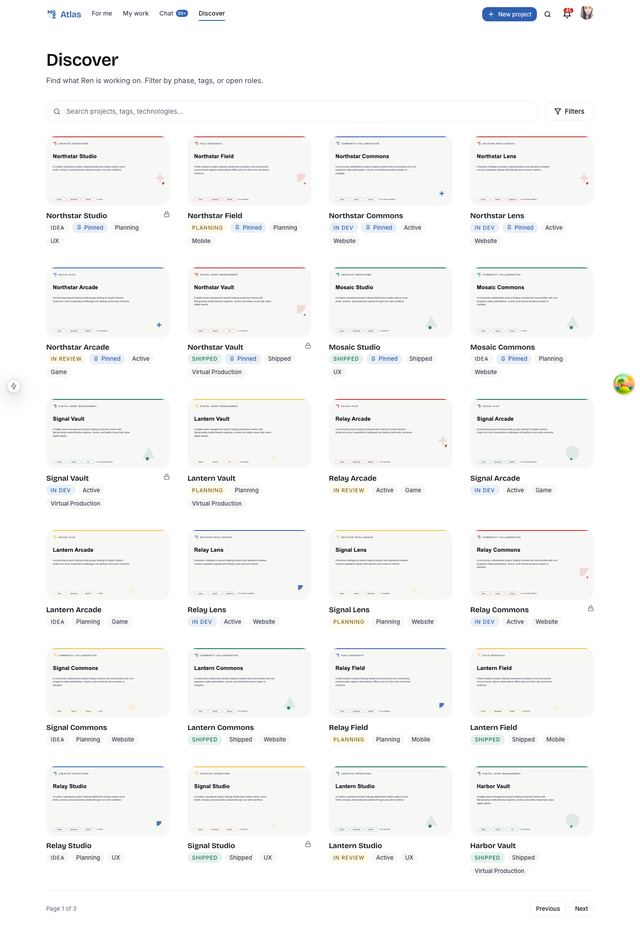
\includegraphics[width=\linewidth]{screenshots/thumbs/063-theme-atlas-light.jpg}\\[0.15em]
{\ttfamily\scriptsize\color{cink3} 063 \quad atlas light}
\end{minipage}
\hfill
\begin{minipage}[t]{0.315\linewidth}
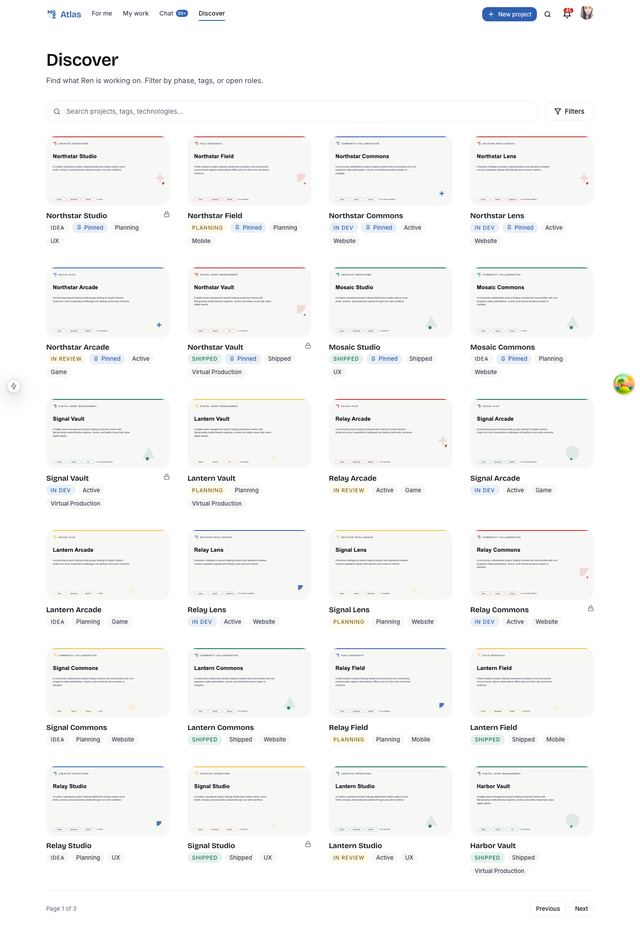
\includegraphics[width=\linewidth]{screenshots/thumbs/064-theme-ocean-light.jpg}\\[0.15em]
{\ttfamily\scriptsize\color{cink3} 064 \quad ocean light}
\end{minipage}
\hfill
\begin{minipage}[t]{0.315\linewidth}
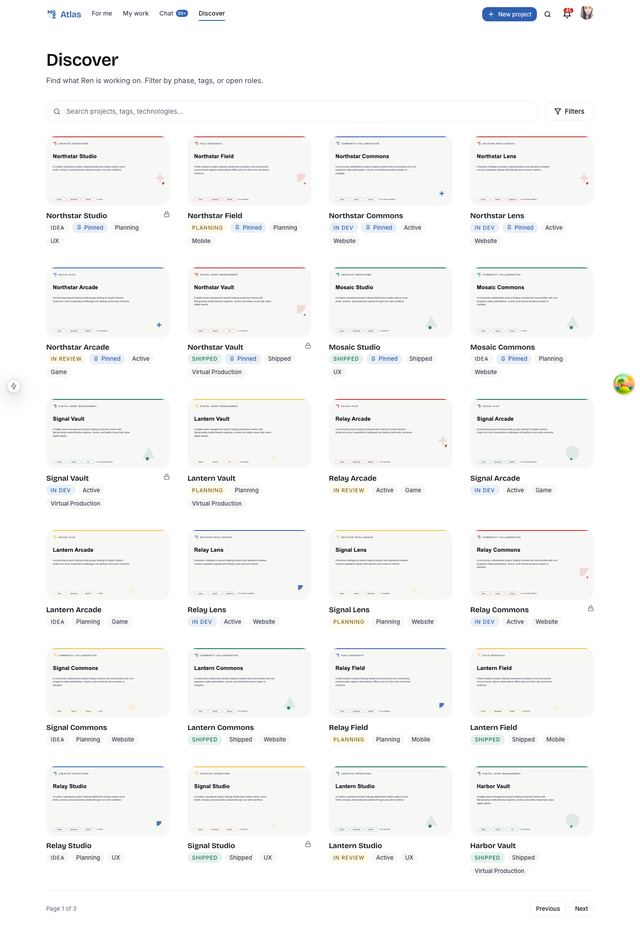
\includegraphics[width=\linewidth]{screenshots/thumbs/065-theme-sunset-light.jpg}\\[0.15em]
{\ttfamily\scriptsize\color{cink3} 065 \quad sunset light}
\end{minipage}
\par\vspace{0.9em}
\noindent
\begin{minipage}[t]{0.315\linewidth}
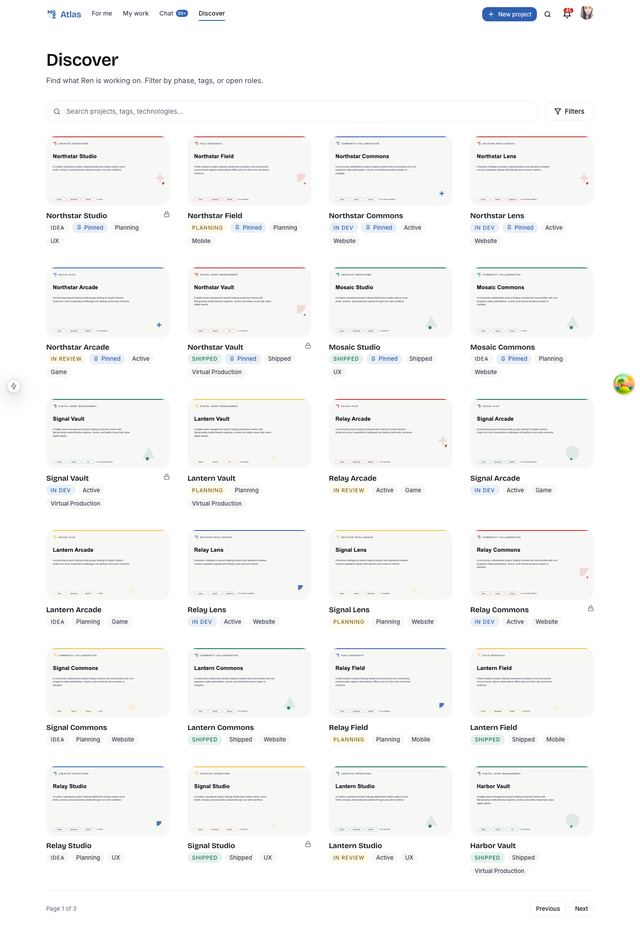
\includegraphics[width=\linewidth]{screenshots/thumbs/066-theme-rose-light.jpg}\\[0.15em]
{\ttfamily\scriptsize\color{cink3} 066 \quad rose light}
\end{minipage}
\hfill
\begin{minipage}[t]{0.315\linewidth}
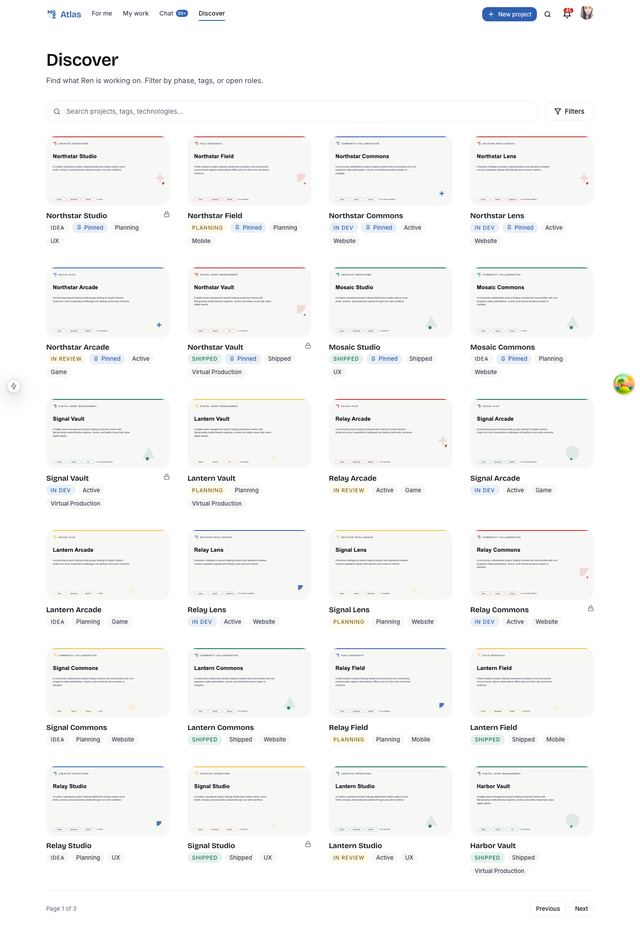
\includegraphics[width=\linewidth]{screenshots/thumbs/067-theme-lavender-light.jpg}\\[0.15em]
{\ttfamily\scriptsize\color{cink3} 067 \quad lavender light}
\end{minipage}
\hfill
\begin{minipage}[t]{0.315\linewidth}
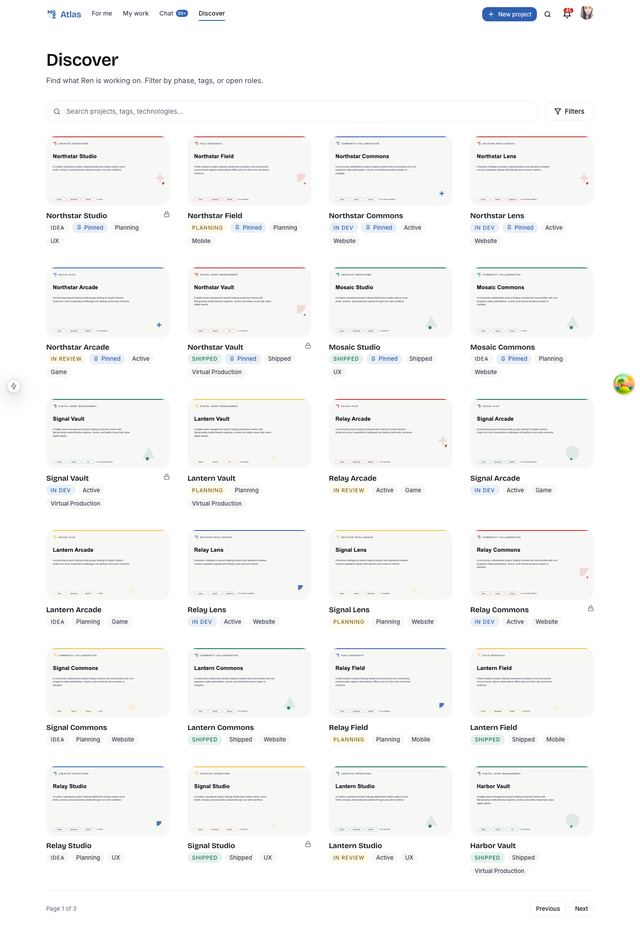
\includegraphics[width=\linewidth]{screenshots/thumbs/068-theme-mint-light.jpg}\\[0.15em]
{\ttfamily\scriptsize\color{cink3} 068 \quad mint light}
\end{minipage}
\par\vspace{0.9em}
\noindent
\begin{minipage}[t]{0.315\linewidth}
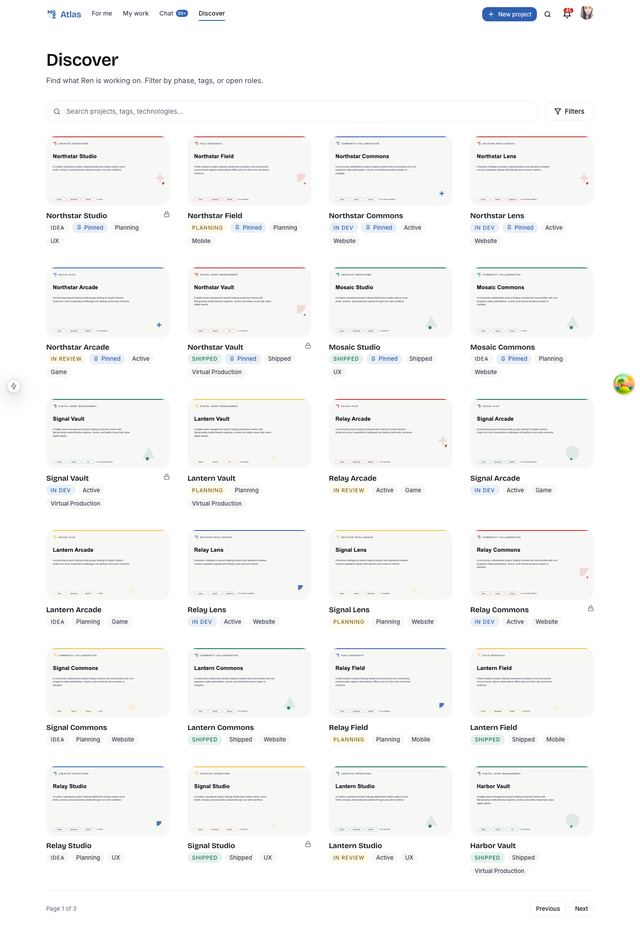
\includegraphics[width=\linewidth]{screenshots/thumbs/069-theme-midnight-dark.jpg}\\[0.15em]
{\ttfamily\scriptsize\color{cink3} 069 \quad midnight dark}
\end{minipage}
\hfill
\begin{minipage}[t]{0.315\linewidth}
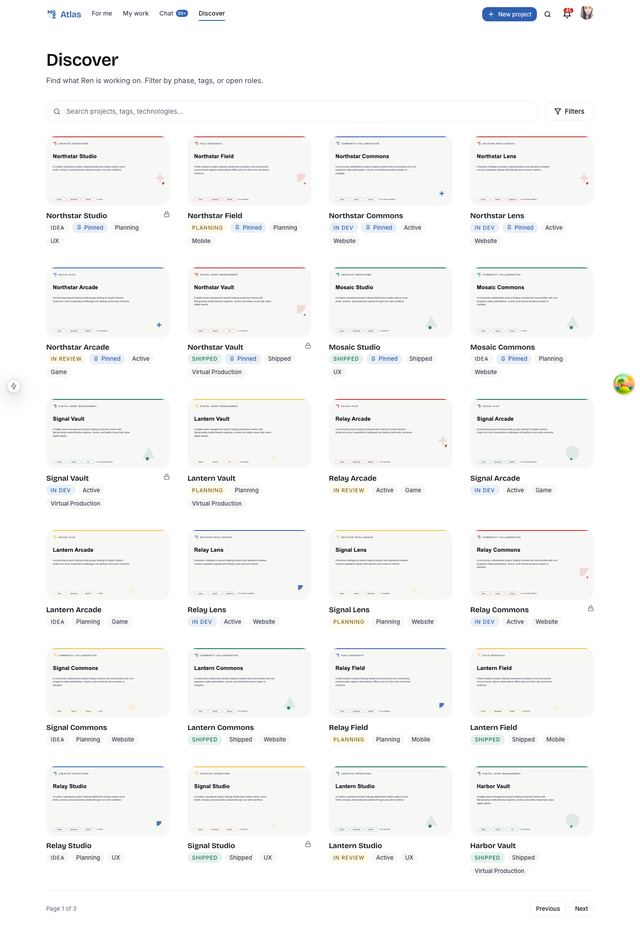
\includegraphics[width=\linewidth]{screenshots/thumbs/070-theme-noir-dark.jpg}\\[0.15em]
{\ttfamily\scriptsize\color{cink3} 070 \quad noir dark}
\end{minipage}

\clearpage
\subsection*{Legal dan Status Sistem}
\vspace{0.3em}
\noindent
\begin{minipage}[t]{0.315\linewidth}
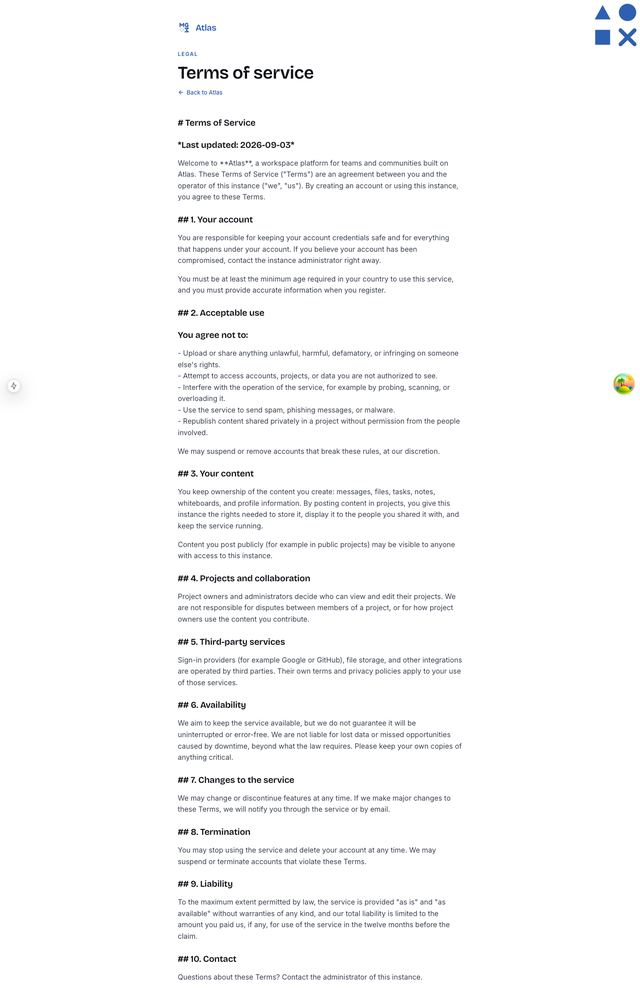
\includegraphics[width=\linewidth]{screenshots/thumbs/071-misc-legal-terms.jpg}\\[0.15em]
{\ttfamily\scriptsize\color{cink3} 071 \quad legal terms}
\end{minipage}
\hfill
\begin{minipage}[t]{0.315\linewidth}
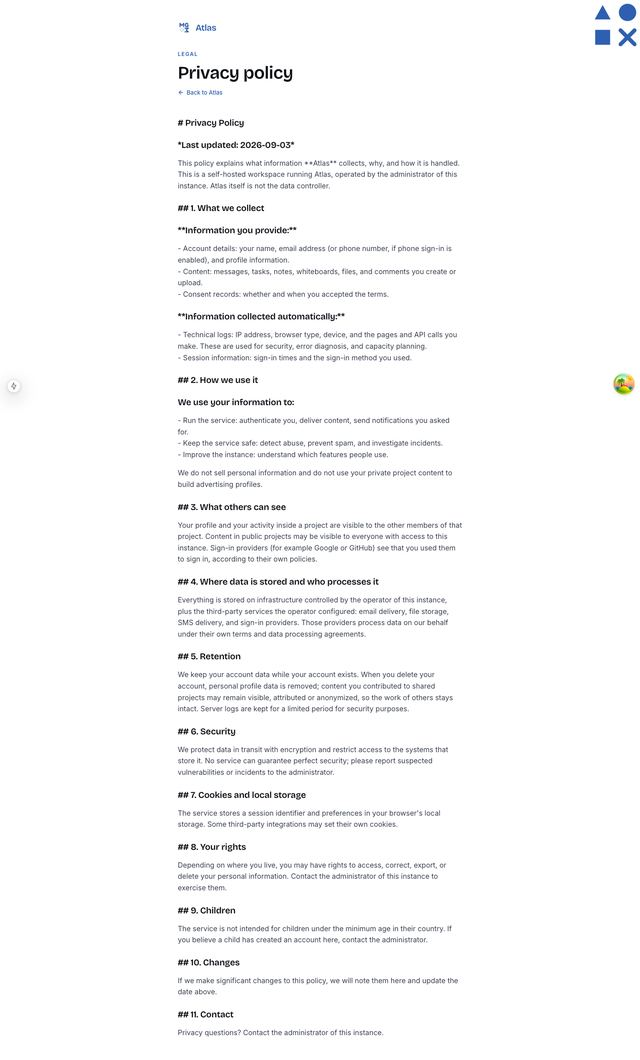
\includegraphics[width=\linewidth]{screenshots/thumbs/072-misc-legal-privacy.jpg}\\[0.15em]
{\ttfamily\scriptsize\color{cink3} 072 \quad legal privacy}
\end{minipage}
\hfill
\begin{minipage}[t]{0.315\linewidth}
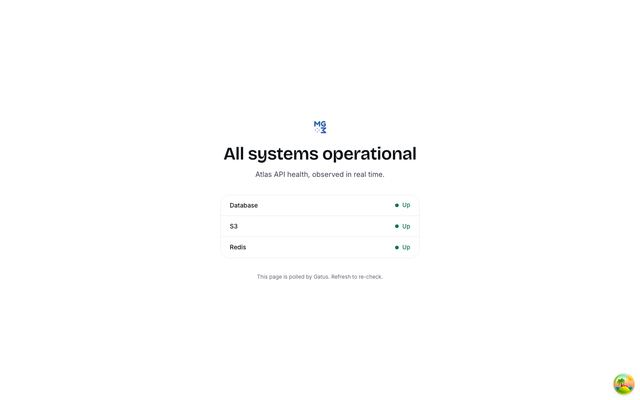
\includegraphics[width=\linewidth]{screenshots/thumbs/073-misc-health.jpg}\\[0.15em]
{\ttfamily\scriptsize\color{cink3} 073 \quad health}
\end{minipage}

\clearpage
\subsection*{Responsif di Layar Ponsel}
\vspace{0.3em}
\noindent
\begin{minipage}[t]{0.315\linewidth}
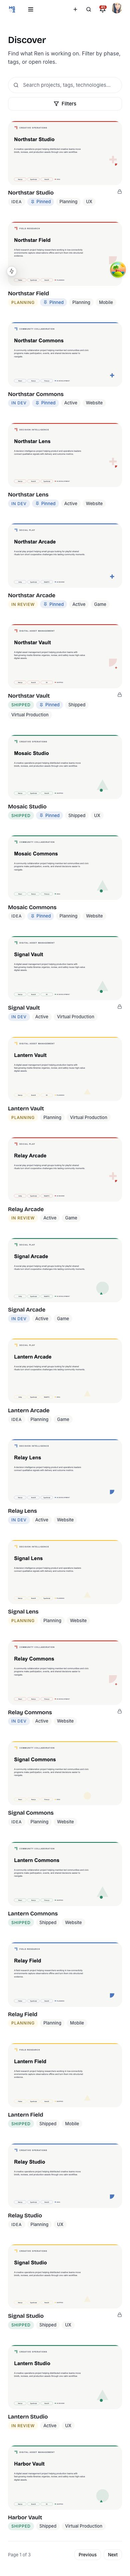
\includegraphics[width=\linewidth]{screenshots/thumbs/074-mobile-dashboard.jpg}\\[0.15em]
{\ttfamily\scriptsize\color{cink3} 074 \quad dashboard}
\end{minipage}
\hfill
\begin{minipage}[t]{0.315\linewidth}
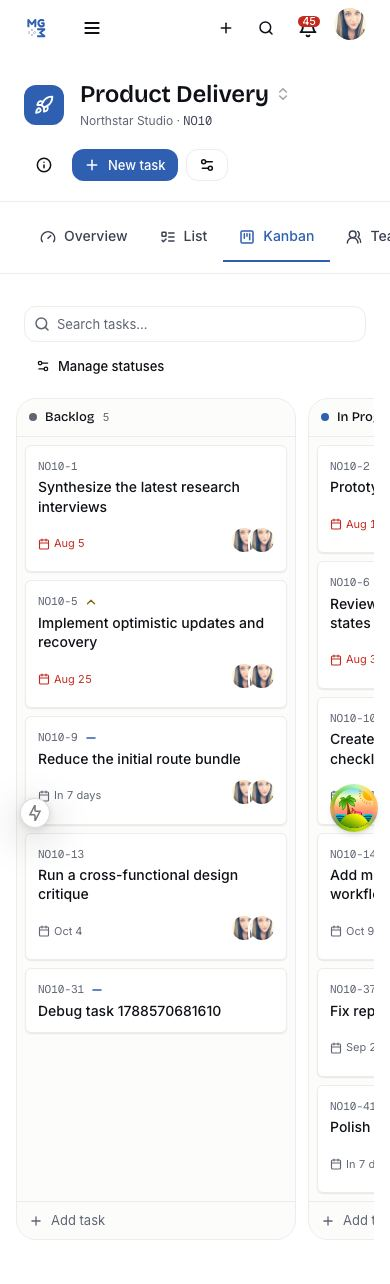
\includegraphics[width=\linewidth]{screenshots/thumbs/075-mobile-kanban.jpg}\\[0.15em]
{\ttfamily\scriptsize\color{cink3} 075 \quad kanban}
\end{minipage}
\hfill
\begin{minipage}[t]{0.315\linewidth}
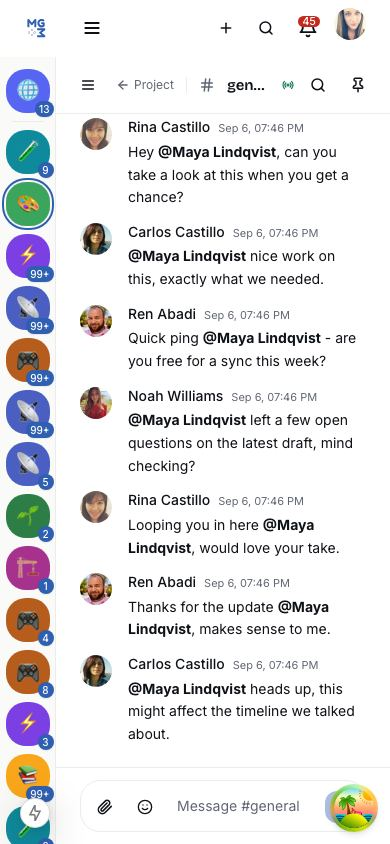
\includegraphics[width=\linewidth]{screenshots/thumbs/076-mobile-chat.jpg}\\[0.15em]
{\ttfamily\scriptsize\color{cink3} 076 \quad chat}
\end{minipage}
\par\vspace{0.9em}
\noindent
\begin{minipage}[t]{0.315\linewidth}
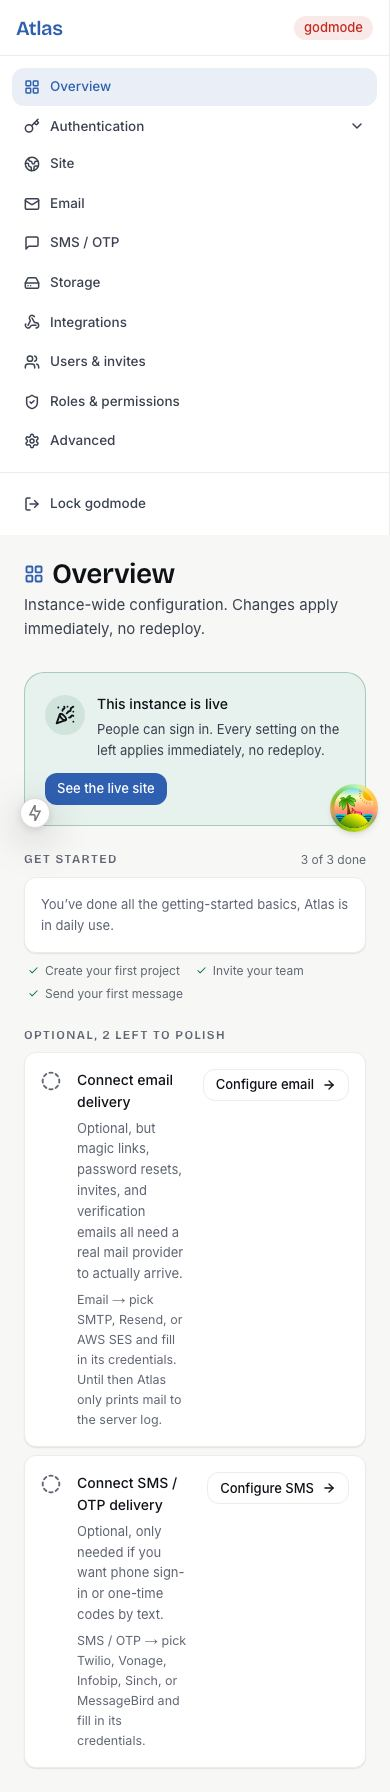
\includegraphics[width=\linewidth]{screenshots/thumbs/077-mobile-godmode.jpg}\\[0.15em]
{\ttfamily\scriptsize\color{cink3} 077 \quad godmode}
\end{minipage}
\hfill
\begin{minipage}[t]{0.315\linewidth}
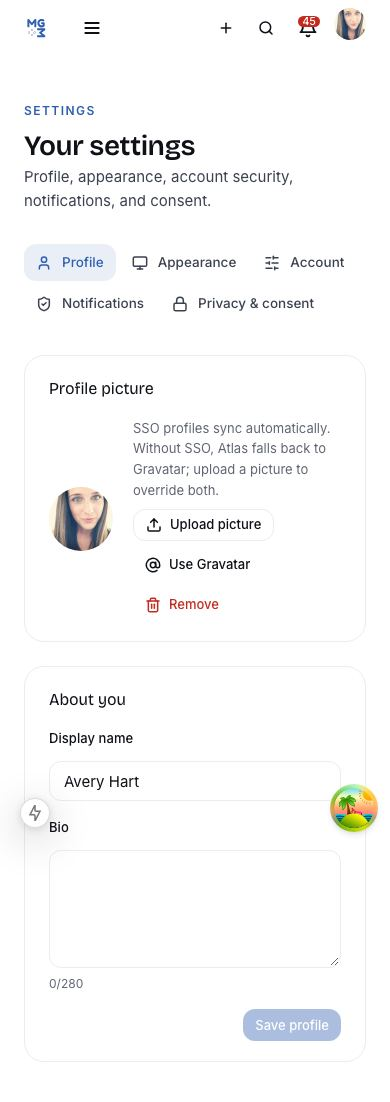
\includegraphics[width=\linewidth]{screenshots/thumbs/078-mobile-settings.jpg}\\[0.15em]
{\ttfamily\scriptsize\color{cink3} 078 \quad settings}
\end{minipage}
\hfill
\begin{minipage}[t]{0.315\linewidth}
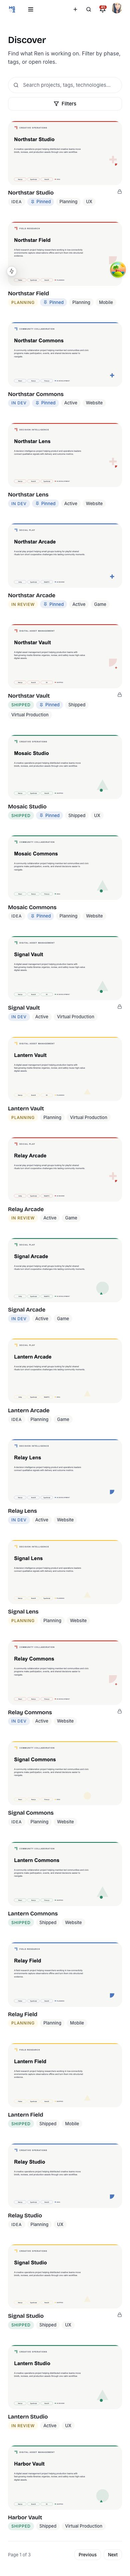
\includegraphics[width=\linewidth]{screenshots/thumbs/079-mobile-projects.jpg}\\[0.15em]
{\ttfamily\scriptsize\color{cink3} 079 \quad projects}
\end{minipage}


\end{document}
